\documentclass{bioinfo_tracer}
\copyrightyear{2017}
\pubyear{2017}

% amsmath package, useful for mathematical formulas
\usepackage{amsmath}
% amssymb package, useful for mathematical symbols
\usepackage{amssymb}

\usepackage{graphicx}
\usepackage{subfigure}
% cite package, to clean up citations in the main text. Do not remove.
\usepackage{cite}

\usepackage{url}

\newcommand{\tracer}{\emph{Tracer}}

\begin{document}
\firstpage{1}

% Title must be 150 characters or less
\title[Tracer]{Posterior summarisation in Bayesian phylogenetics using Tracer 1.7}

\author[Rambaut \textit{et~al.}]{
Andrew Rambaut\,$^{1}$,
Alexei J.~Drummond\,$^{2,3}$,
Dong Xie\,$^{2,3}$,
Guy Baele$^{4}$,
Marc A.~Suchard\,$^{5,6}$
}

\address{
$^{1}$Institute of Evolutionary Biology, University of Edinburgh, Edinburgh, UK \\
$^{2}$Department of Computer Science, University of Auckland, Auckland, NZ \\
$^{3}$Centre for Computational Evolution, University of Auckland, Auckland, NZ \\
$^{4}$Department of Microbiology and Immunology, Rega Institute, KU Leuven, Leuven, Belgium\\
$^{5}$Department of Human Genetics, University of California, Los Angeles, USA \\
$^{6}$Department of Biostatistics, University of California, Los Angeles, USA \\
%$^{7}$Department of Human Genetics, David Geffen School of Medicine at UCLA, University of California, Los Angeles, USA\\
}

\history{Received on XXXXX; revised on XXXXX; accepted on XXXXX}

\editor{Associate Editor: XXXXXXX}

\maketitle


% Please keep the abstract between 250 and 300 words
\begin{abstract}

\section{Motivation:}
Bayesian inference of phylogeny using Markov chain Monte Carlo (MCMC) plays a central role in understanding evolutionary history from molecular sequence data.
Visualising and analysing the MCMC-generated samples from the posterior distribution is a key step in any non-trivial Bayesian inference. %, and it is especially important for methods that employ MCMC.
\section{Results:}
We present the software package \tracer\ (version 1.7) for visualising and analysing the MCMC trace files generated through Bayesian phylogenetic inference.
\tracer\ provides kernel density estimation, multivariate visualisation, demographic trajectory reconstruction, conditional posterior distribution summary and more.
\section{Availability:}
\tracer\ is open-source and available at \url{http://beast.community/tracer}.

\section{Contact:}
\href{a.rambaut@ed.ac.uk}{\url{a.rambaut@ed.ac.uk}},
\href{alexei@cs.auckland.ac.nz}{\url{alexei@cs.auckland.ac.nz}}
and
\href{msuchard@ucla.edu}{\url{msuchard@ucla.edu}}

\end{abstract}

\section*{Introduction}

Bayesian inference of phylogeny using Markov chain Monte Carlo (MCMC) \citep{rannala1996probability, mau1999bayesian, drummond2002estimating} flourishes as a popular approach to uncover the evolutionary relationships among taxa, such as genes, genomes, individuals or species.
MCMC approaches generate samples of model parameter values - including the phylogenetic tree - drawn from their posterior distribution given molecular sequence data and a selection of evolutionary models.
Visualising, tabulating and marginalising these samples is critical for approximating the posterior quantities of interest that one reports as the outcome of a Bayesian phylogenetic analysis.
To facilitate this task, we have developed the \tracer\ (version 1.7) software package to
process MCMC trace files containing parameter samples and to interactively explore the high-dimensional posterior distribution.
\tracer\ works automatically with sample output from BEAST \citep{drummond2012bayesian}, BEAST2 \citep{bouckaert2014beast2},  LAMARC \citep{kuhner2006lamarc},  Migrate \citep{beerli2006comparison}, MrBayes \citep{ronquist2012mrbayes}, RevBayes \citep{hohna2016revbayes} and possibly other MCMC programs from other domains.

\section*{Design and Implementation}

%A key feature of \tracer\ is its ability to link together samples from quantitative model parameter trace files with tree trace files. %% AR - only for the demographic reconstructions...
%This linkage is not available in other popular post-processing MCMC software, such as coda \citep{plummer2006coda} and AWTY \citep{nylander2007awty}, and enables users to approximate the posterior distribution of scientifically relevant quantities that are functions of both the tree and other quantitative measures. %% AR - ... which are intended in these other software packages.
For each trace, \tracer\ examines the posterior samples from all the available parameters, treating continuous, integer and categorical parameters appropriately, and presents statistical summaries and visualizations.
Further, \tracer\ can analyse a single trace or combine samples from multiple files.
Immediately apparent in the default \tracer\ view, the effective sample size (ESS) is one such statistic that
allows users to assess the number of effectively independent draws from the posterior distribution the trace represents (Figure \ref{fig:overview}:a).
Colour coding assists the user in determining potential MCMC mixing problems, with cut-off values at 100 and 200.

%\tracer\ is able to handle three trace types, also known as variable types \citep{mendenhall2012introduction}: real, integer, and categorical.
%The real trace type is used to handle quantitative continuous variables, which commonly appear in phylodynamic analyses, whereas the integer trace type allows to deal with quantitative discrete variables and the categorical trace is meant for qualitative categorical variables.
%The three trace types are automatically assigned when the trace file is imported but can also manually be set.

Selecting multiple parameters from the ``Traces" panel on the left generates a side-by-side comparison or an overlay of the selected parameters' visualisations (Figure \ref{fig:overview}:b-e).
Multiple trace files can be selected in a similar fashion to compare posterior samples between different replicates of an analysis.
If multiple trace files have the same file name,  then a ``Combined'' trace appears automatically.
% , which can be selected as well as the individual trace files.
\tracer\ generates four display panels for the selected parameters:


\begin{itemize}

\item Estimates: Reports common summary statistics such as the sample mean, standard deviation, highest posterior density interval and ESS.  Also presents a histogram of sample values for a single selected parameter (Figure \ref{fig:overview}:a) or  side-by-side boxplots for multiple continuous parameters (Figure \ref{fig:overview}:b).

\item Marginal Density: Draws density plots for the selected parameter(s), including  kernel density estimates (Figure \ref{fig:overview}:c), histograms and violin plots (Figure \ref{fig:overview}:d) for continuous parameters and frequency plots for categorical or integer parameters.

\item Joint-Marginal: Visualisation in this panel appears after selecting two or more parameters and the plot form depends on the parameter types. We show several examples in the next section of the paper.

\item Trace: Constructs line plots connecting the sequential samples of one or more selected parameters against state or generation number (Figure \ref{fig:overview}:e).  Users typically use this plot to assess mixing, select a suitable burn-in and identify trends that suggest convergence issues.
\end{itemize}
%

%
\begin{figure}[t]
\subfigure[Tracer overview]{\hspace{0.40cm}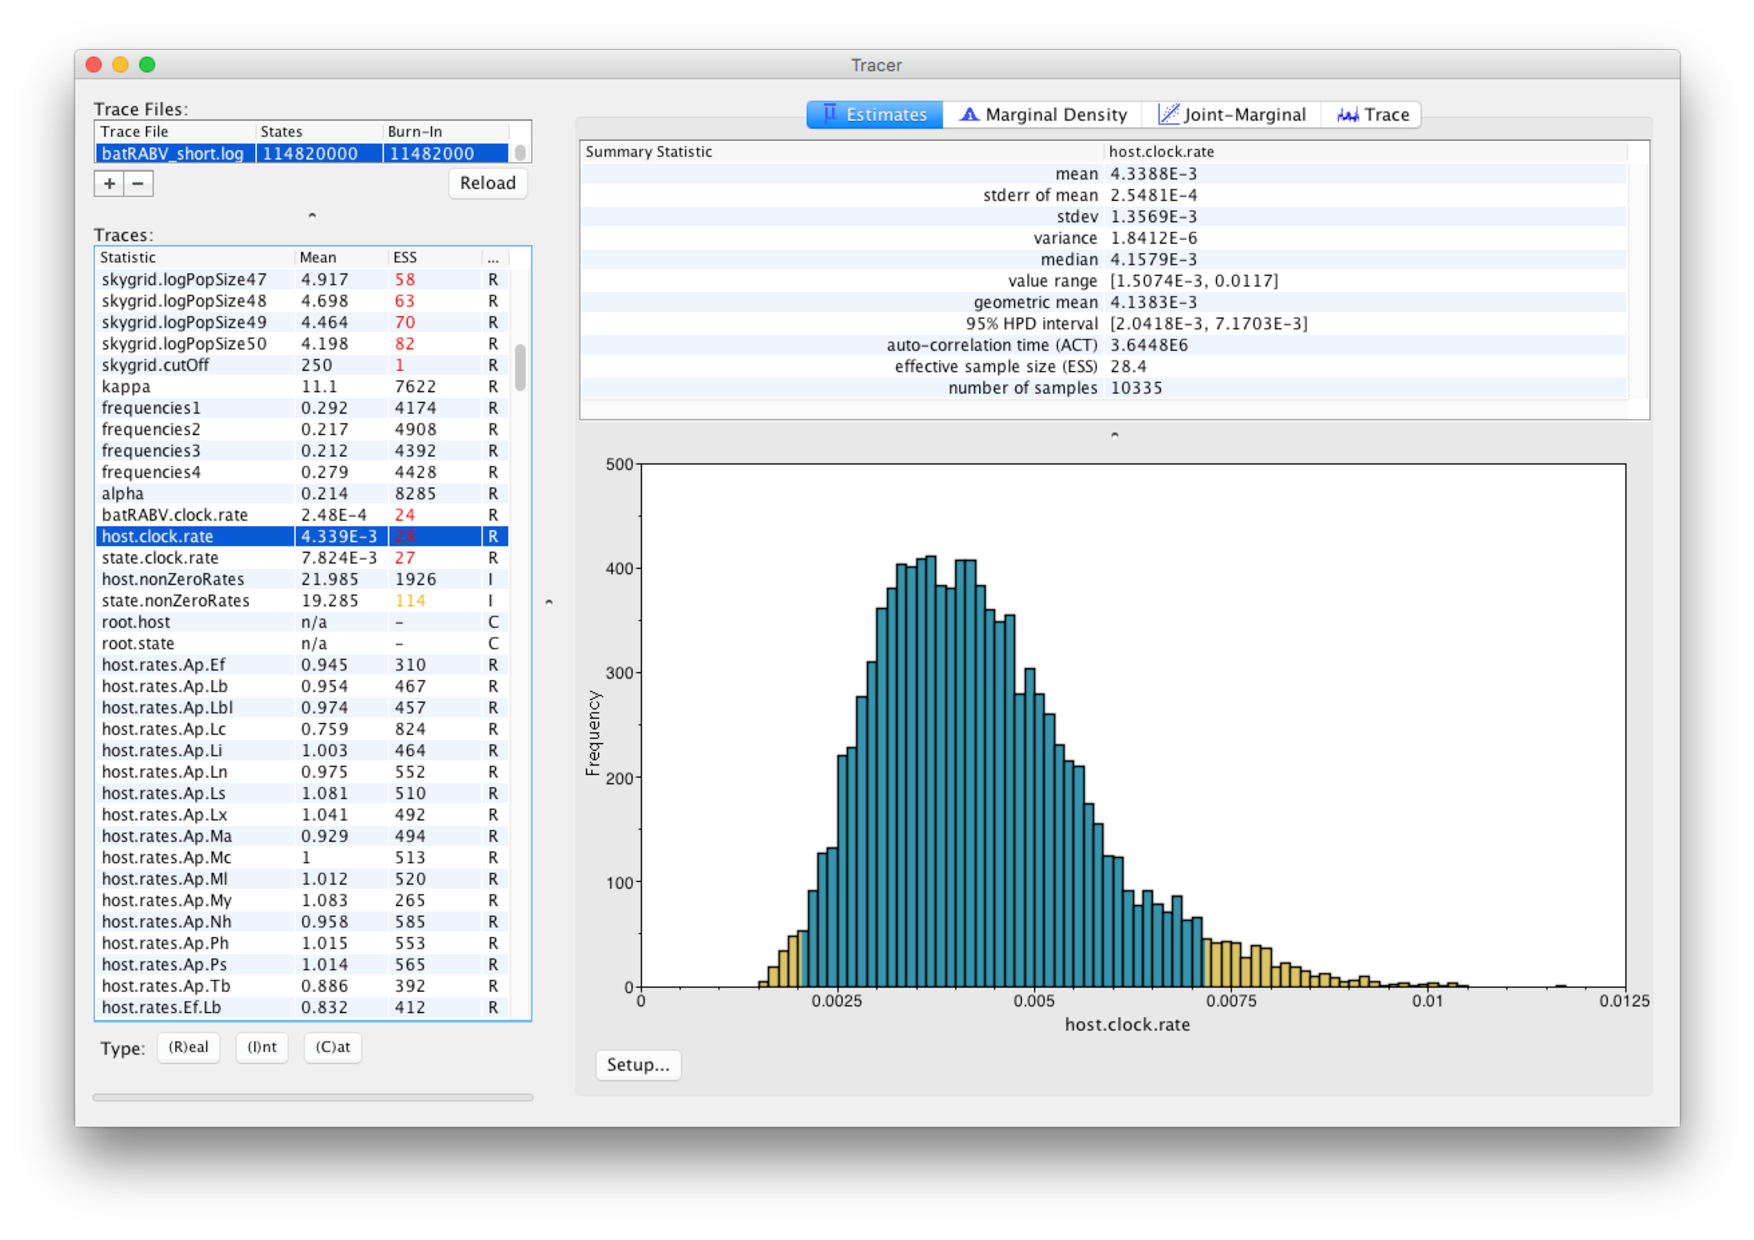
\includegraphics[width=0.432\textwidth]{./figures/rabv-overview-3.pdf}}
\subfigure[Boxplot]{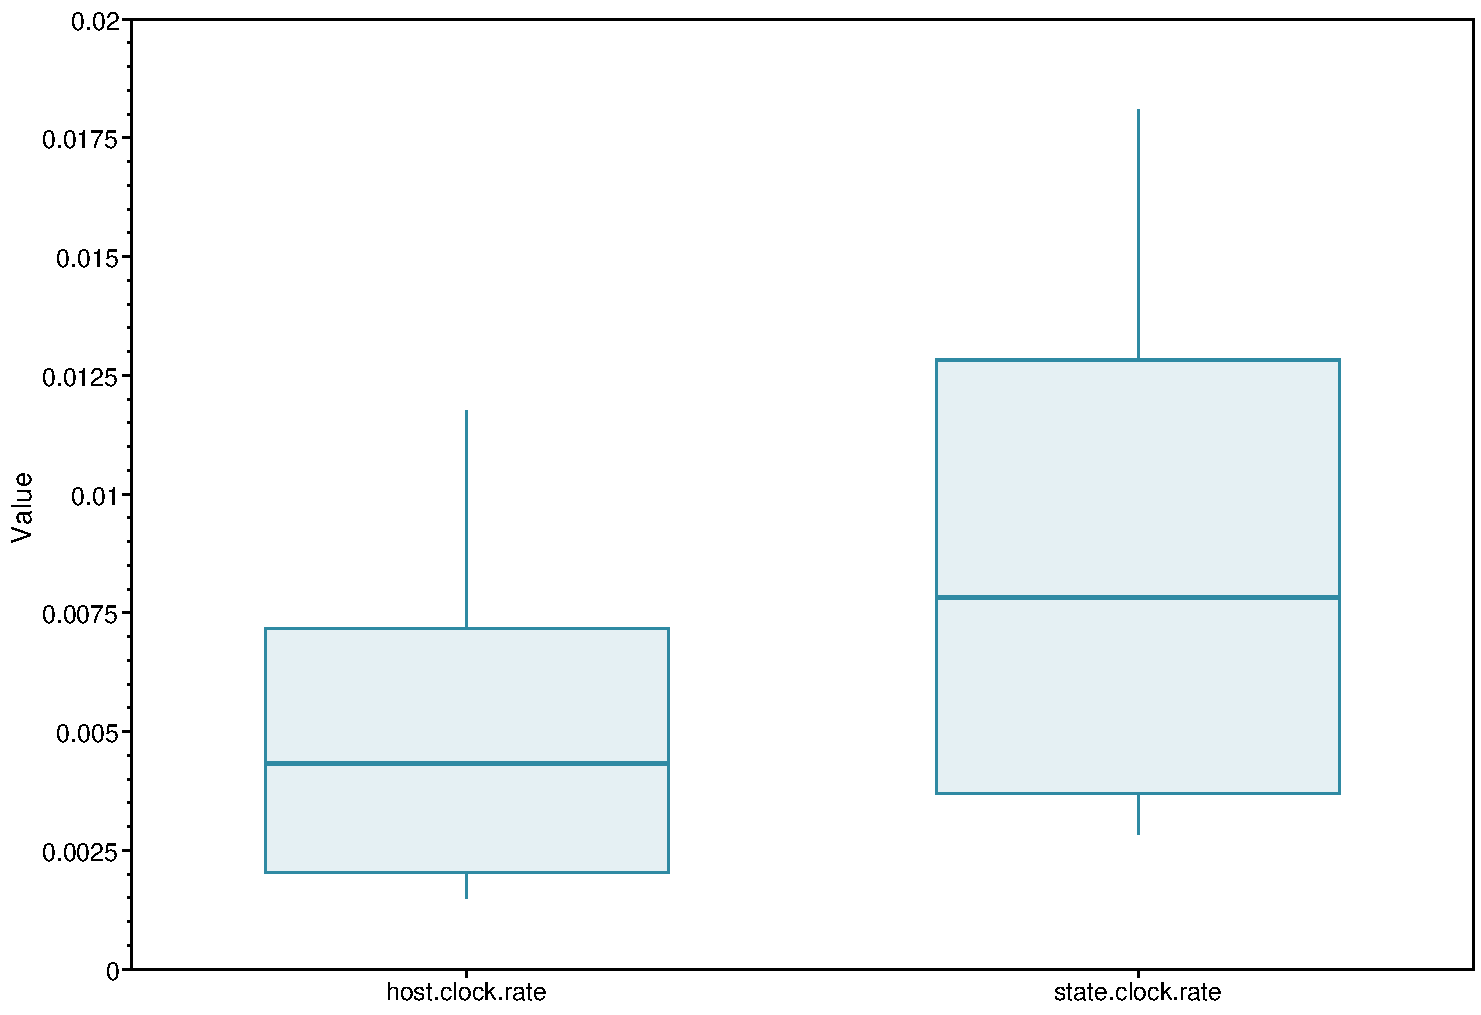
\includegraphics[width = .23\textwidth, height = 3cm]{./figures/rabv-boxplots.pdf}}
\subfigure[Density]{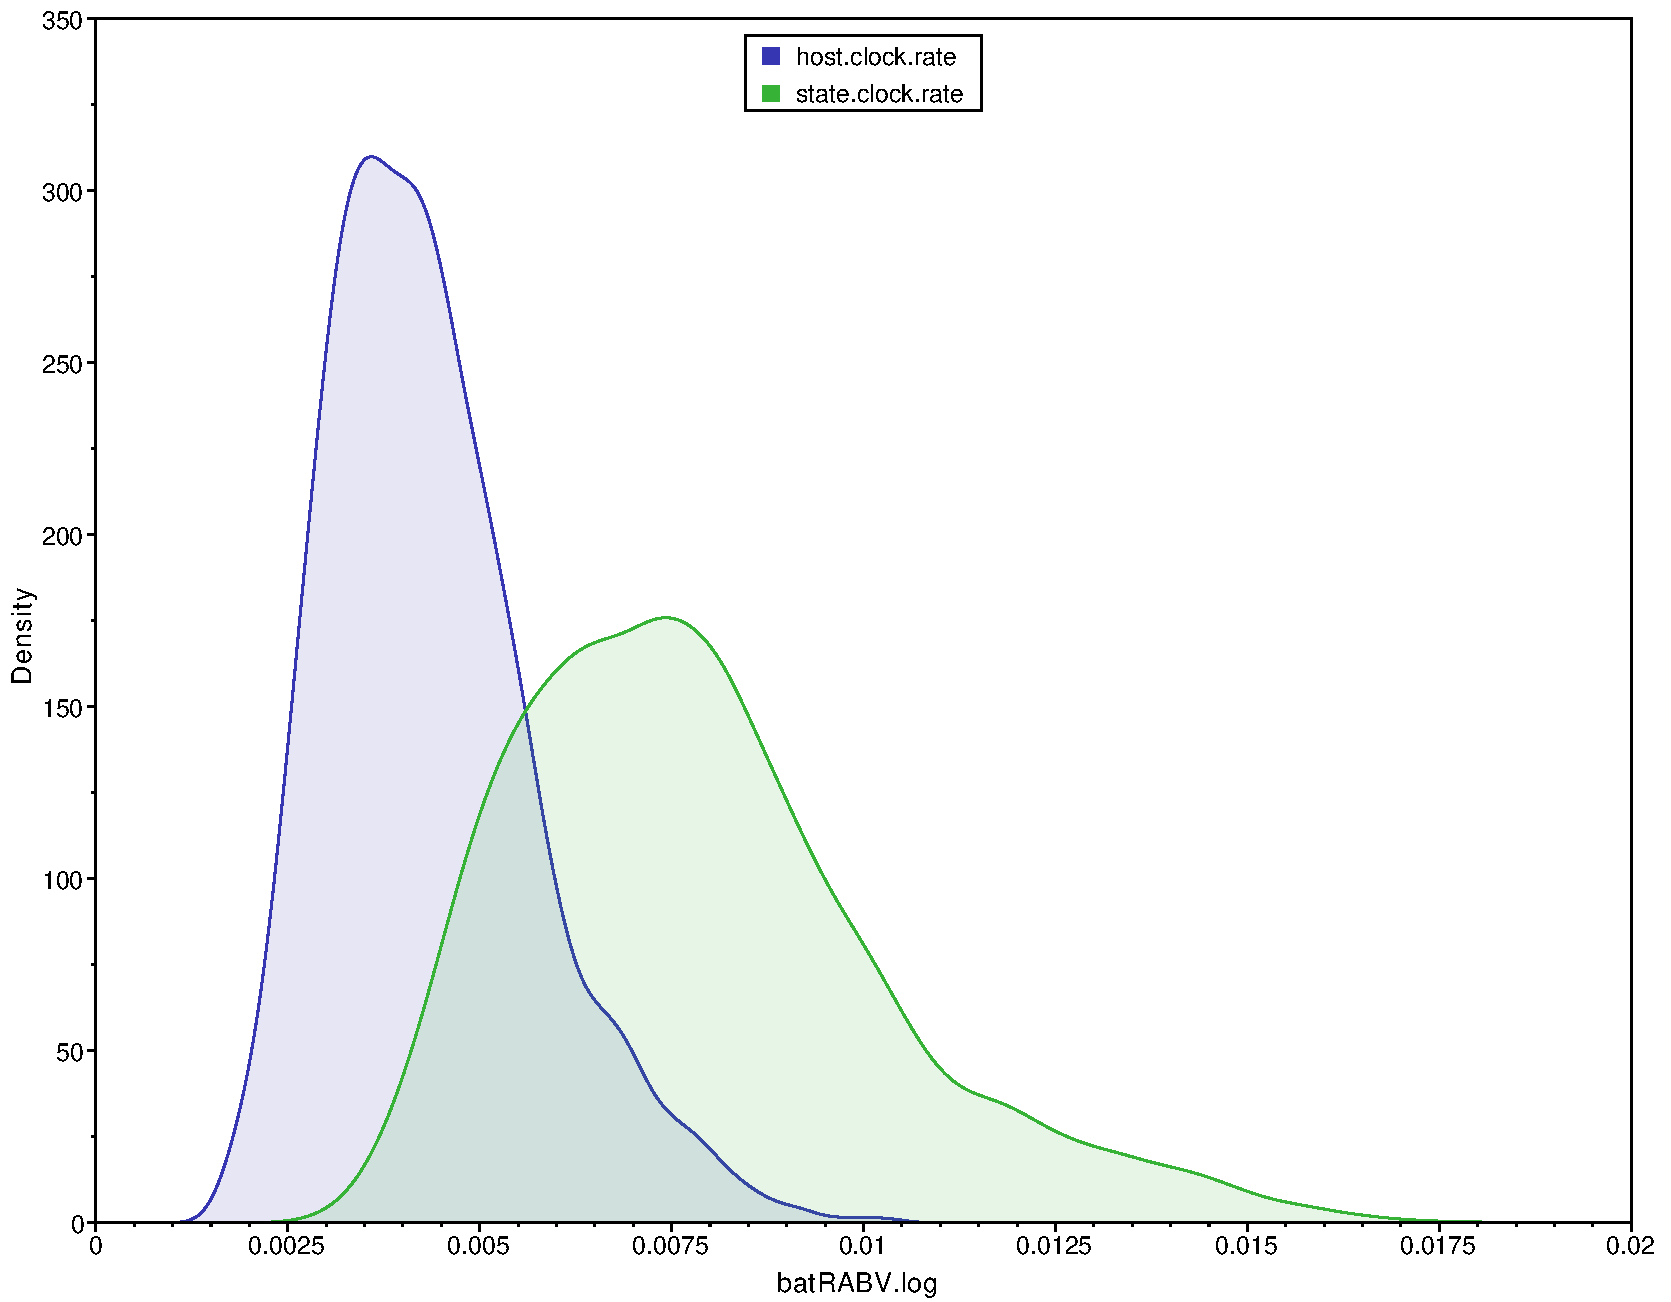
\includegraphics[width = .23\textwidth, height = 3cm]{./figures/rabv-density.pdf}}\\
\subfigure[Violin]{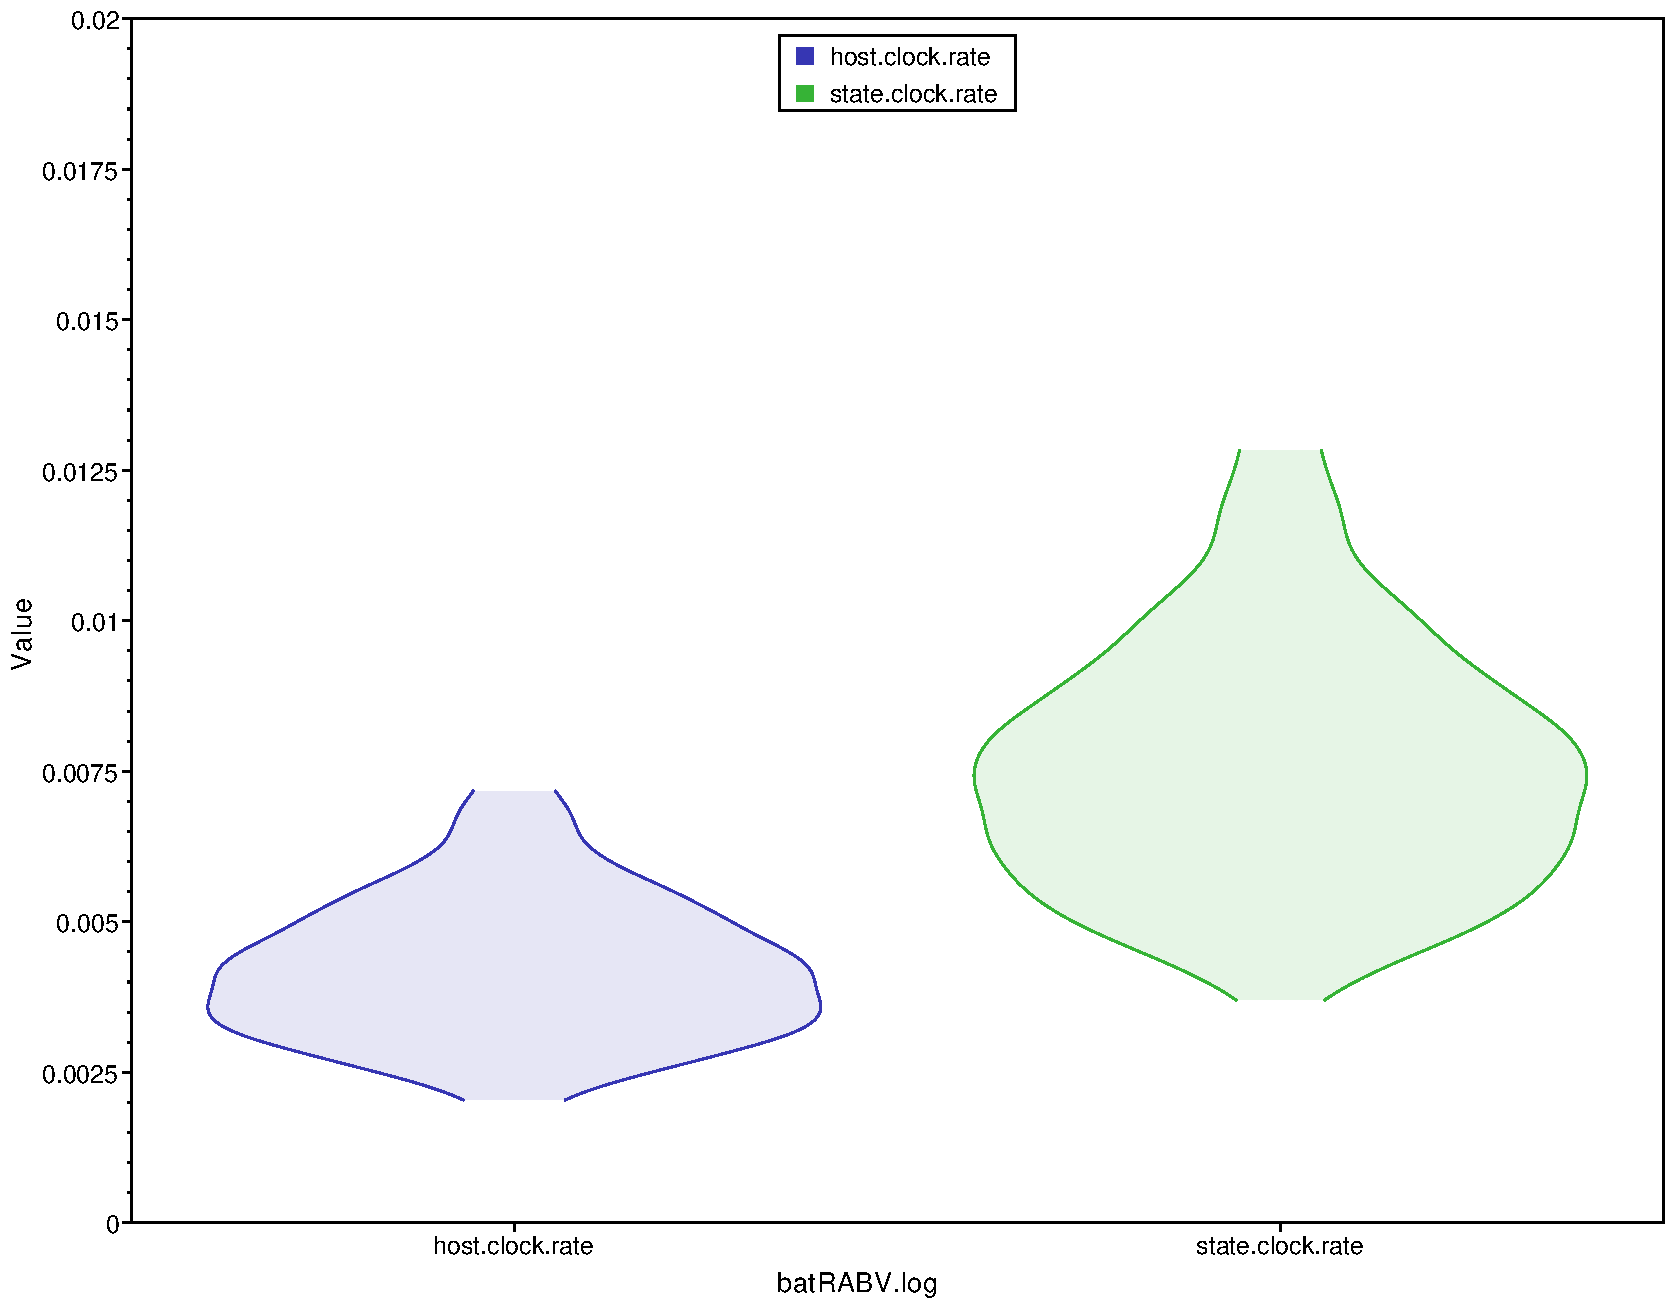
\includegraphics[width = .23\textwidth, height = 3cm]{./figures/rabv-violin.pdf}}
\subfigure[Trace]{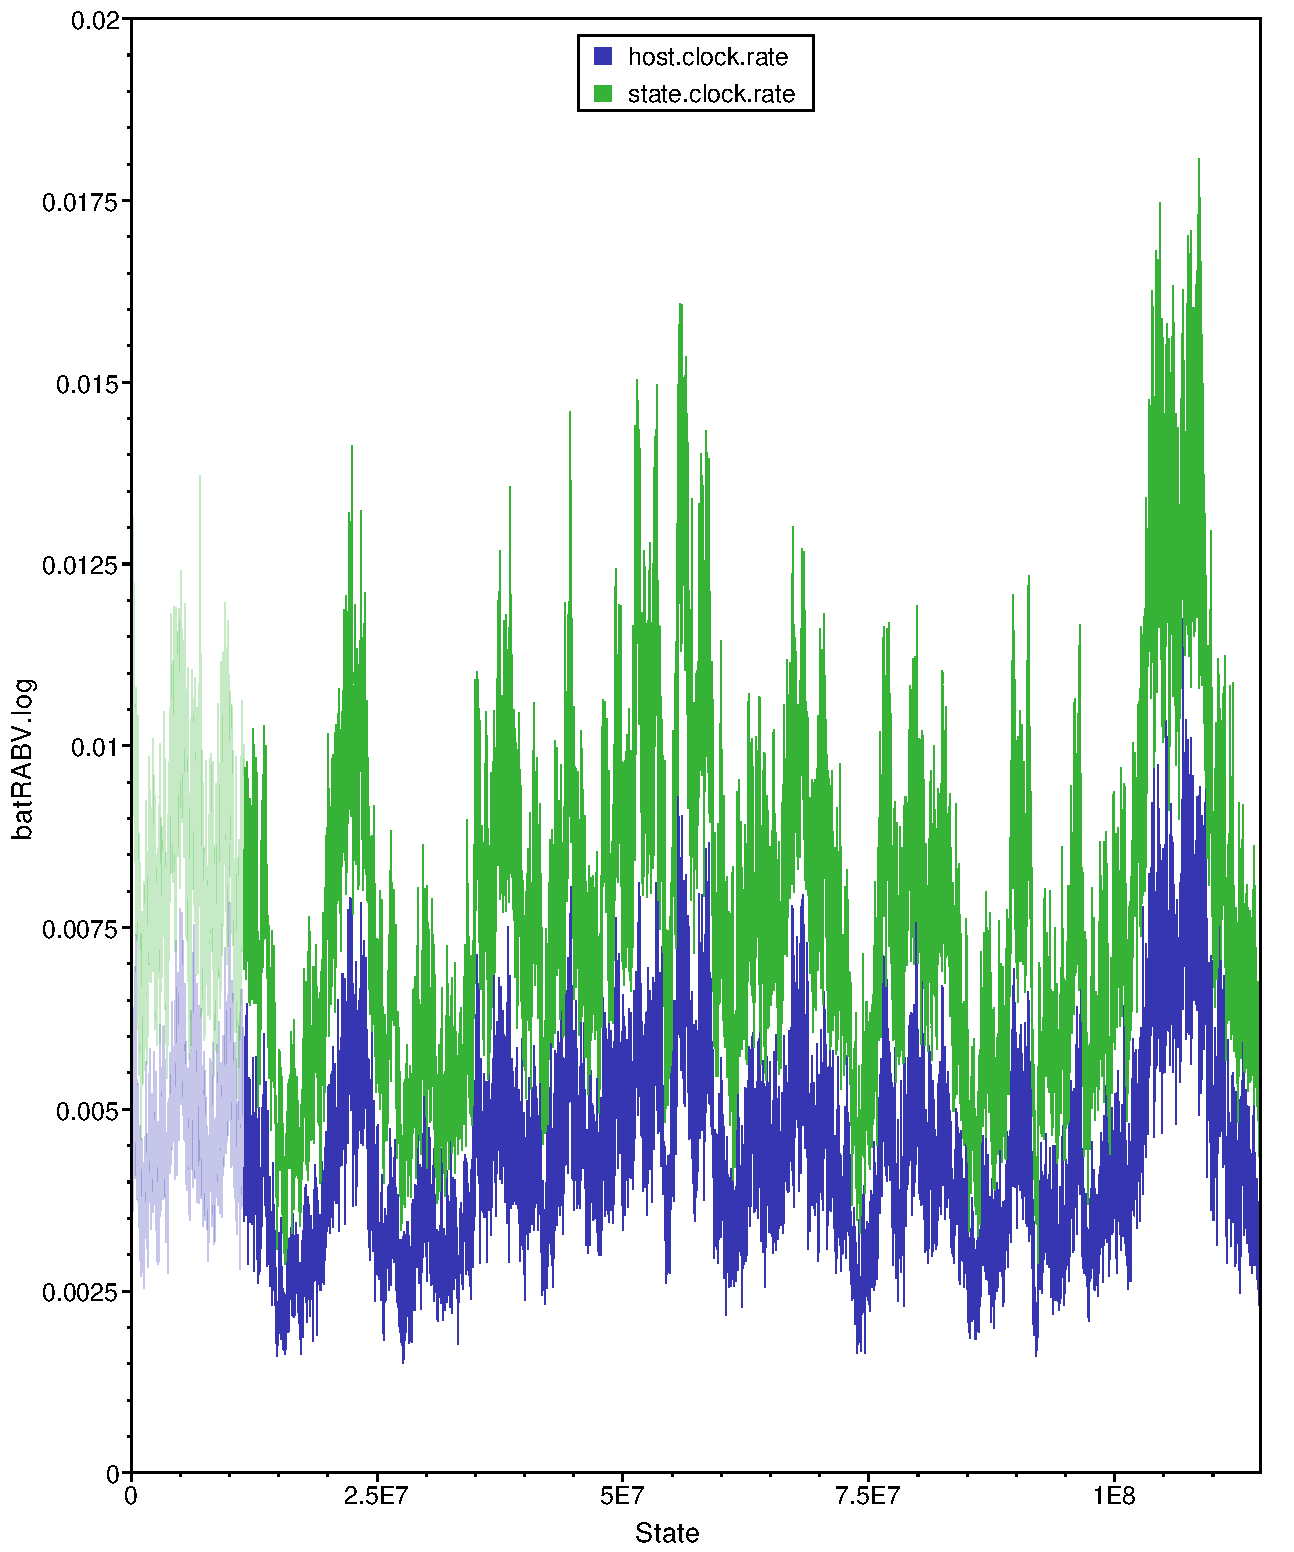
\includegraphics[width = .23\textwidth, height = 3cm]{./figures/rabv-traces.pdf}}
\vspace{-0.25cm}
\caption{Overview of \tracer\ functionality and individual parameter visualisations: (a) Main \tracer\ panel upon loading a single trace file; (b) boxplot representation of two continuous parameters; (c) kernel density estimates; (d) violin plots; (e) the actual traces connecting the parameter values visited by the Markov chain.}
\label{fig:overview}
\end{figure}
%

%
\begin{figure}[t]
\subfigure[Bubble chart]{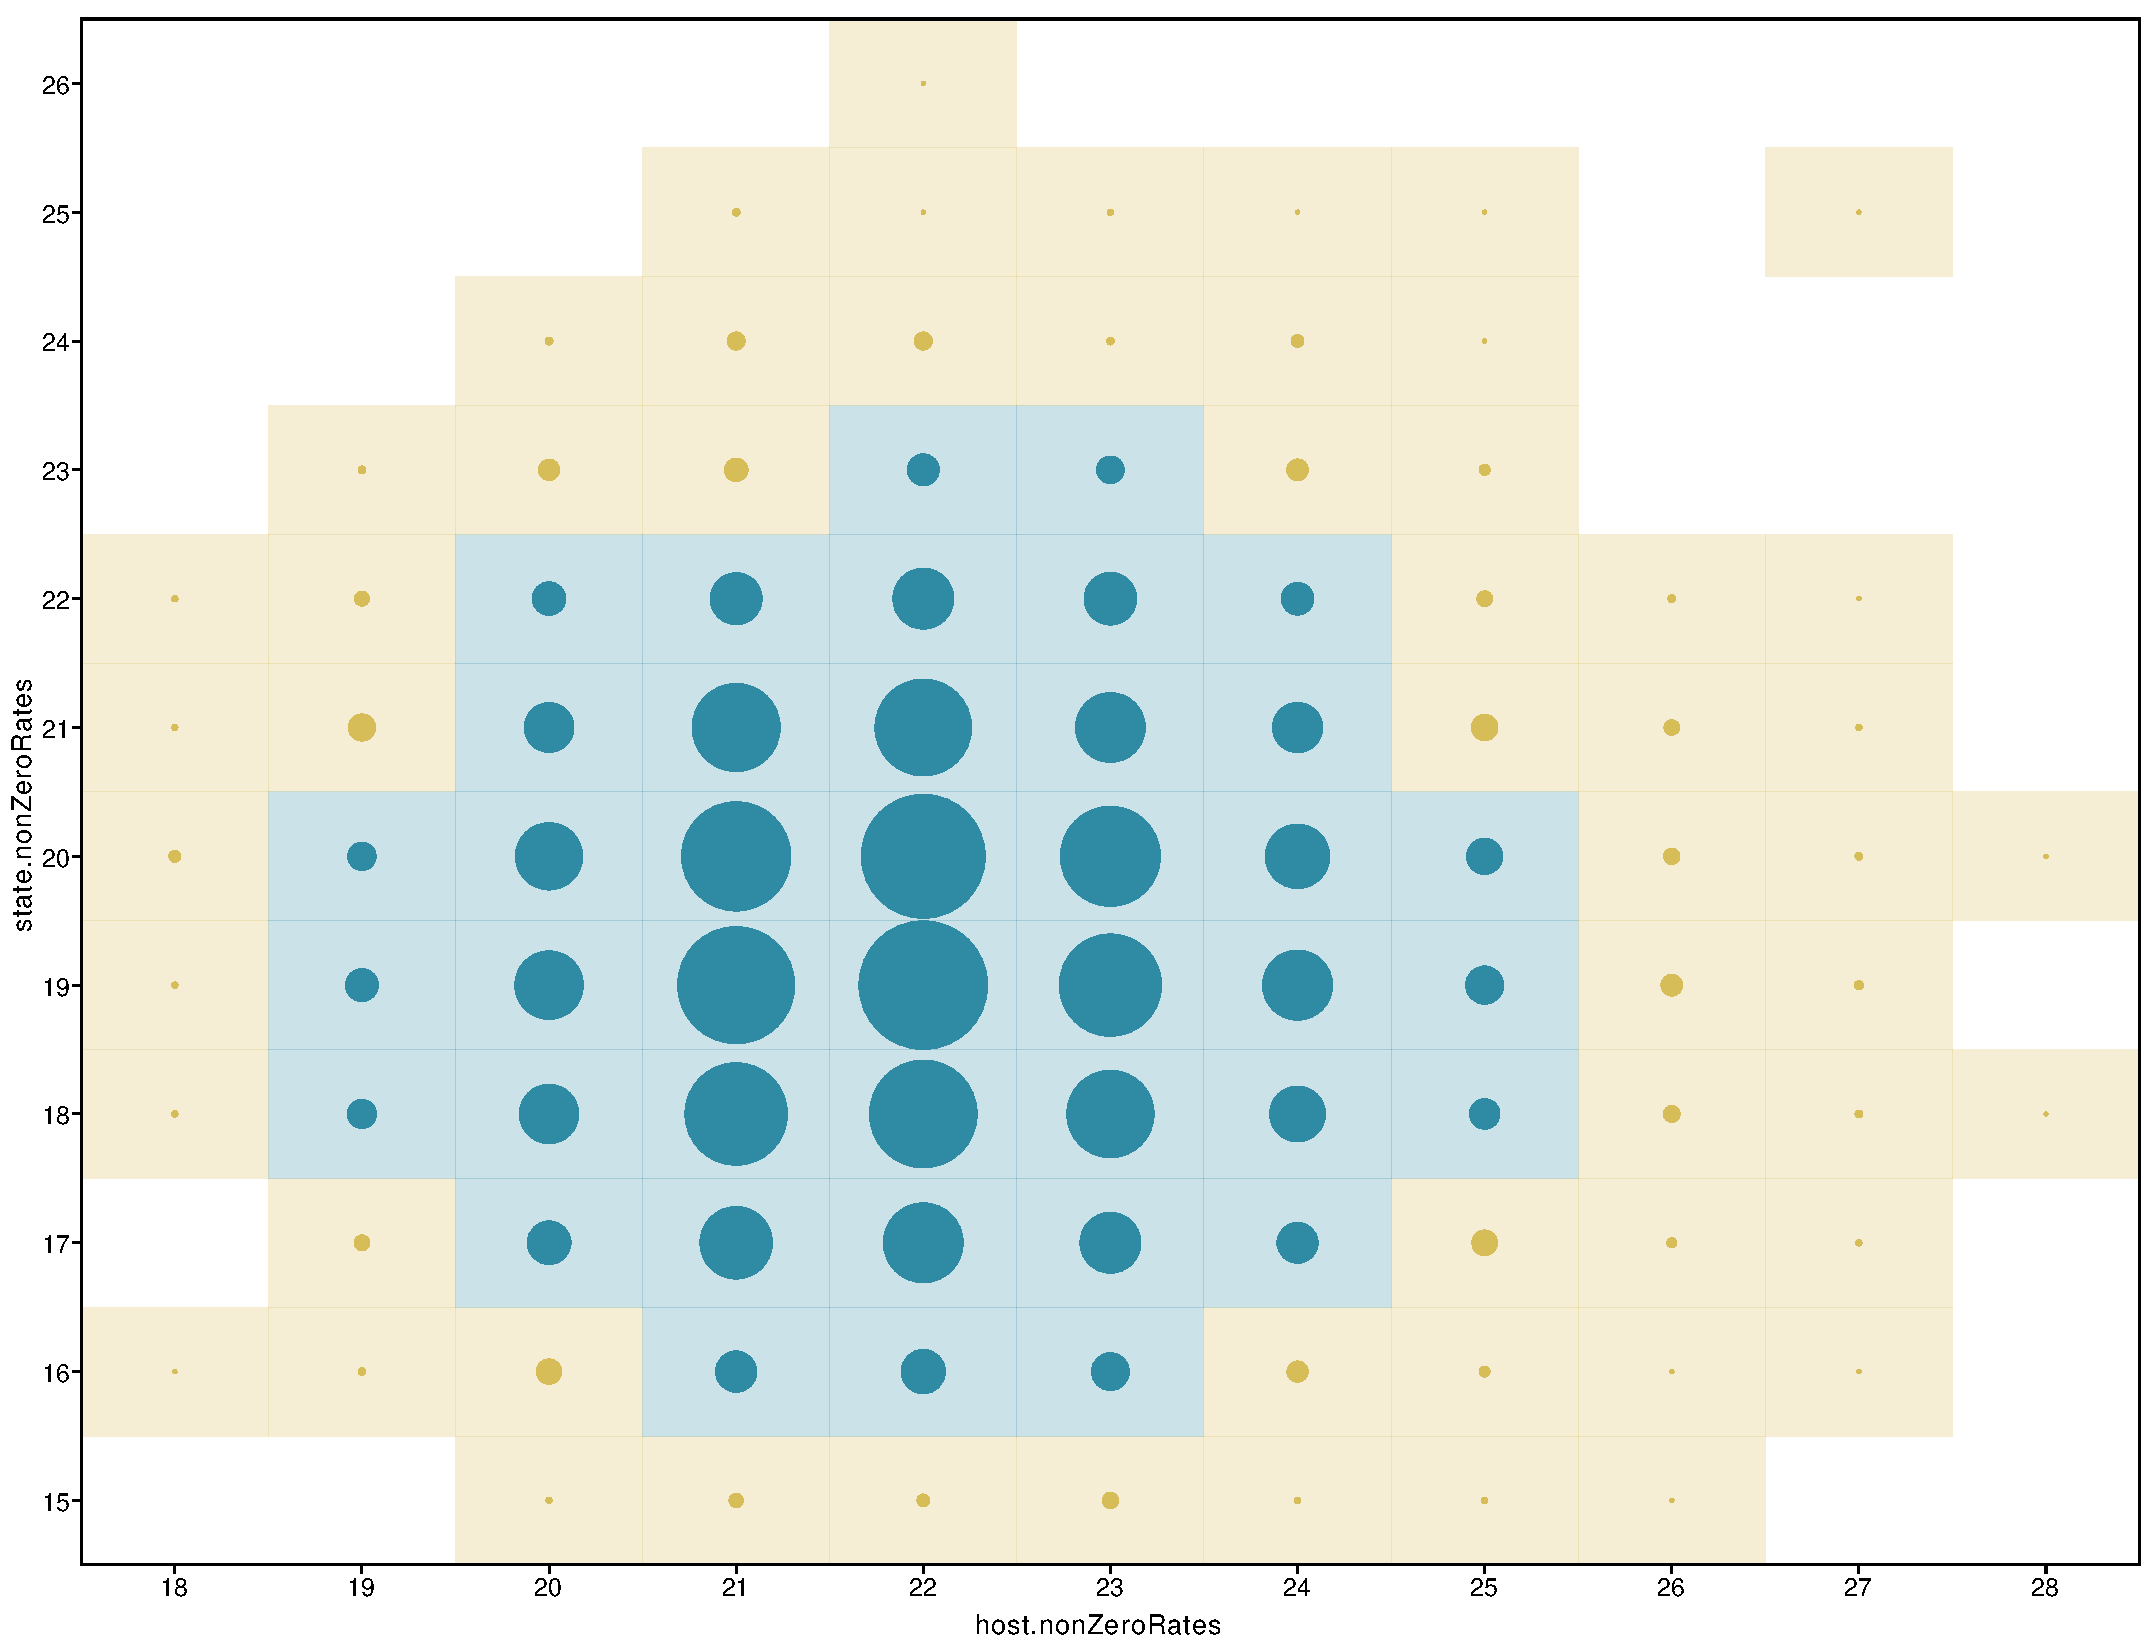
\includegraphics[width = .23\textwidth, height = 3cm]{./figures/rabv-integerjointmarginal-2.pdf}}
\subfigure[Marginal density]{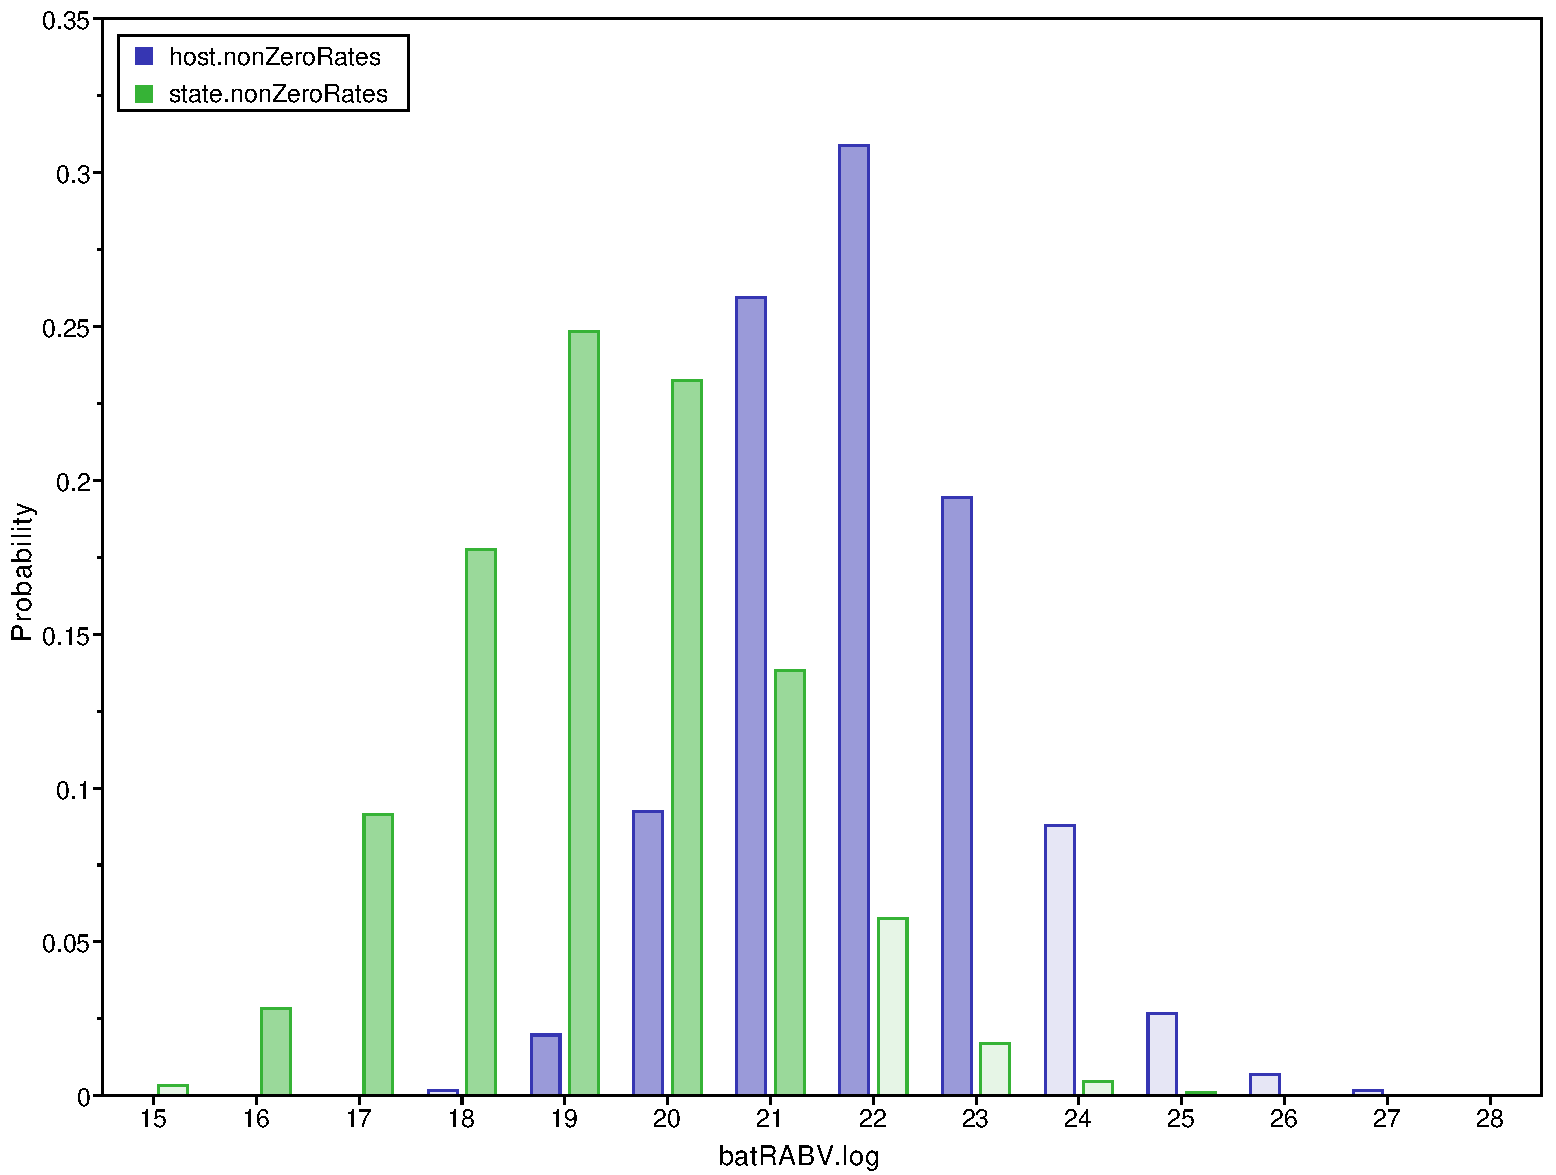
\includegraphics[width = .23\textwidth, height = 3cm]{./figures/rabv-integermarginaldensity.pdf}} \\
\subfigure[Scatter plot]{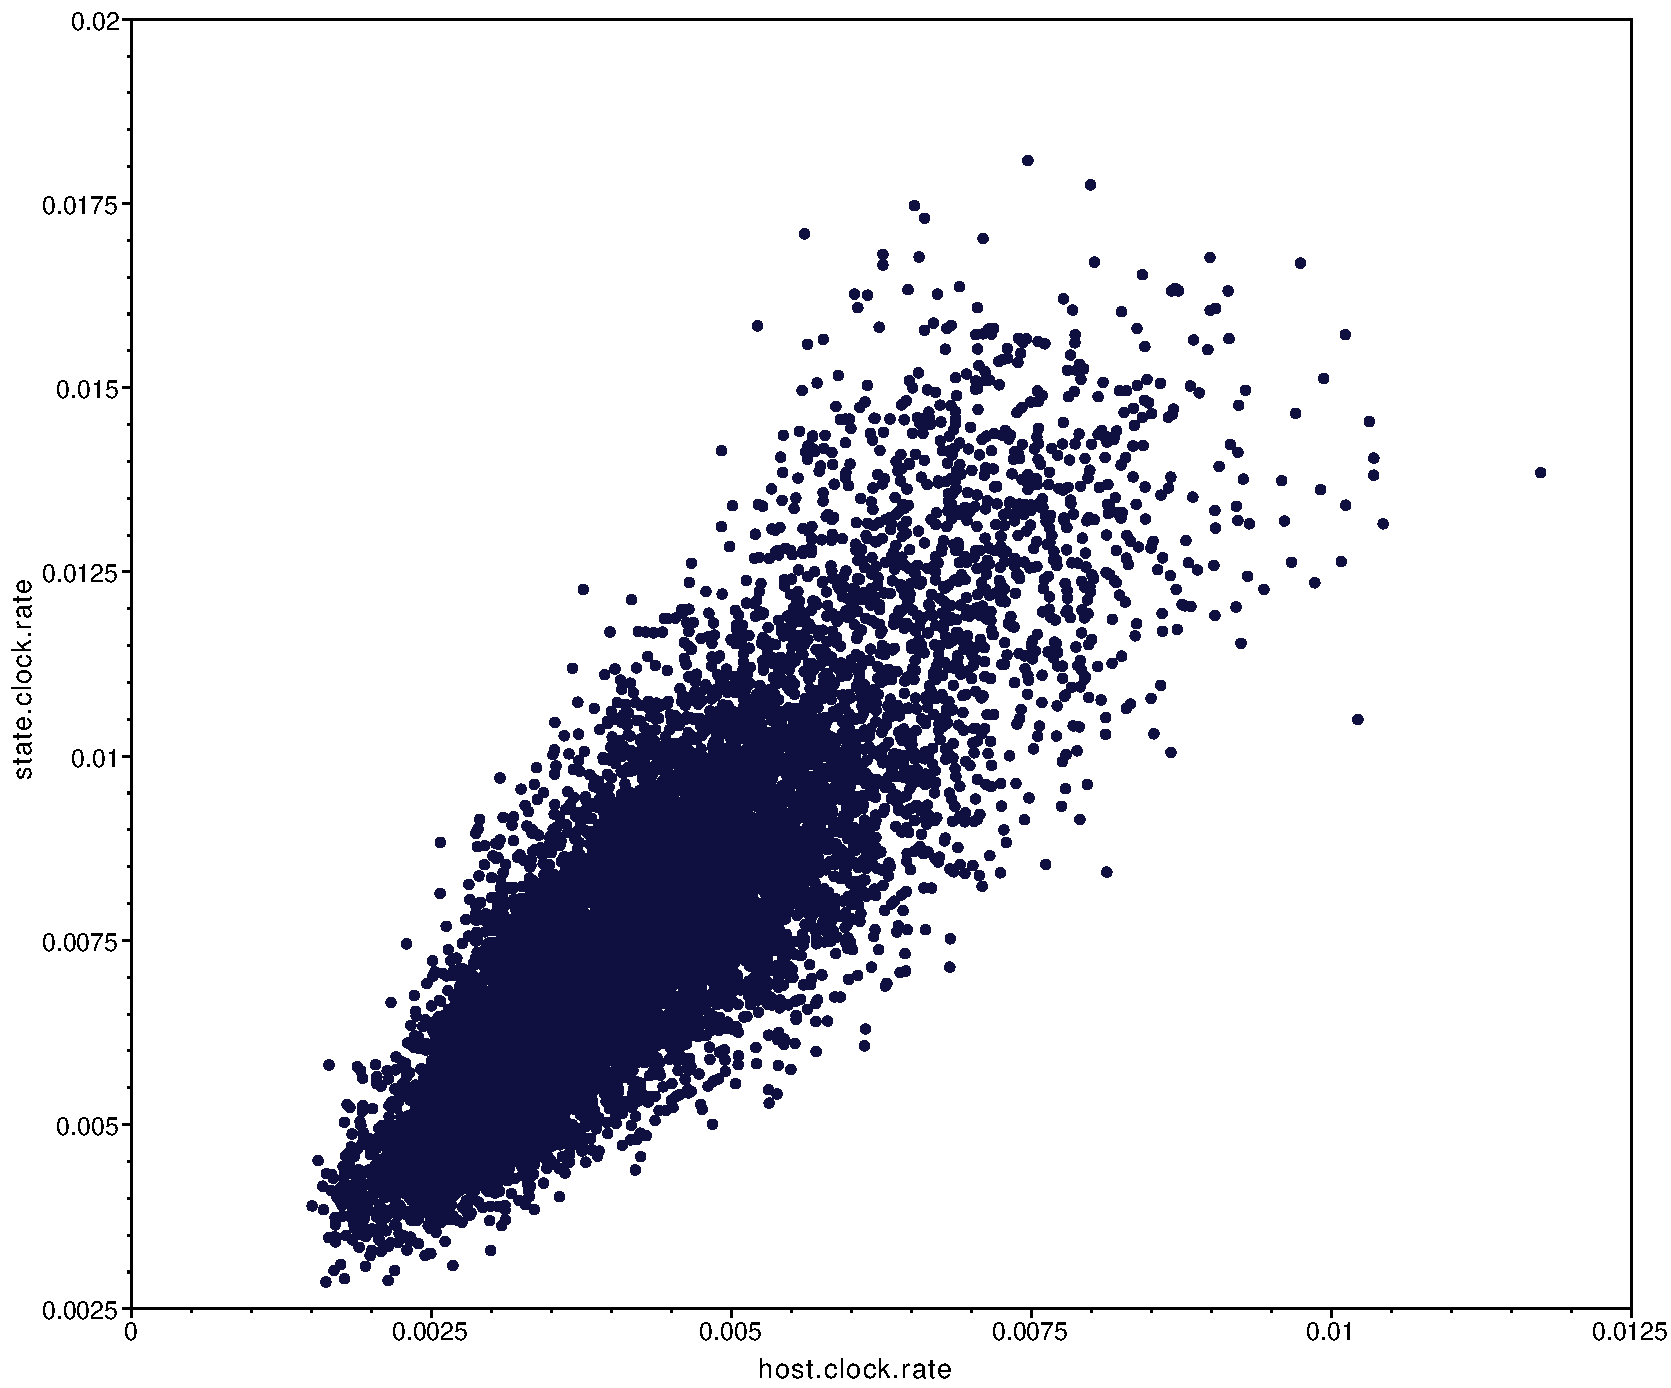
\includegraphics[width = .23\textwidth, height = 3cm]{./figures/rabv-correlation.pdf}}
\subfigure[Correlation plot]{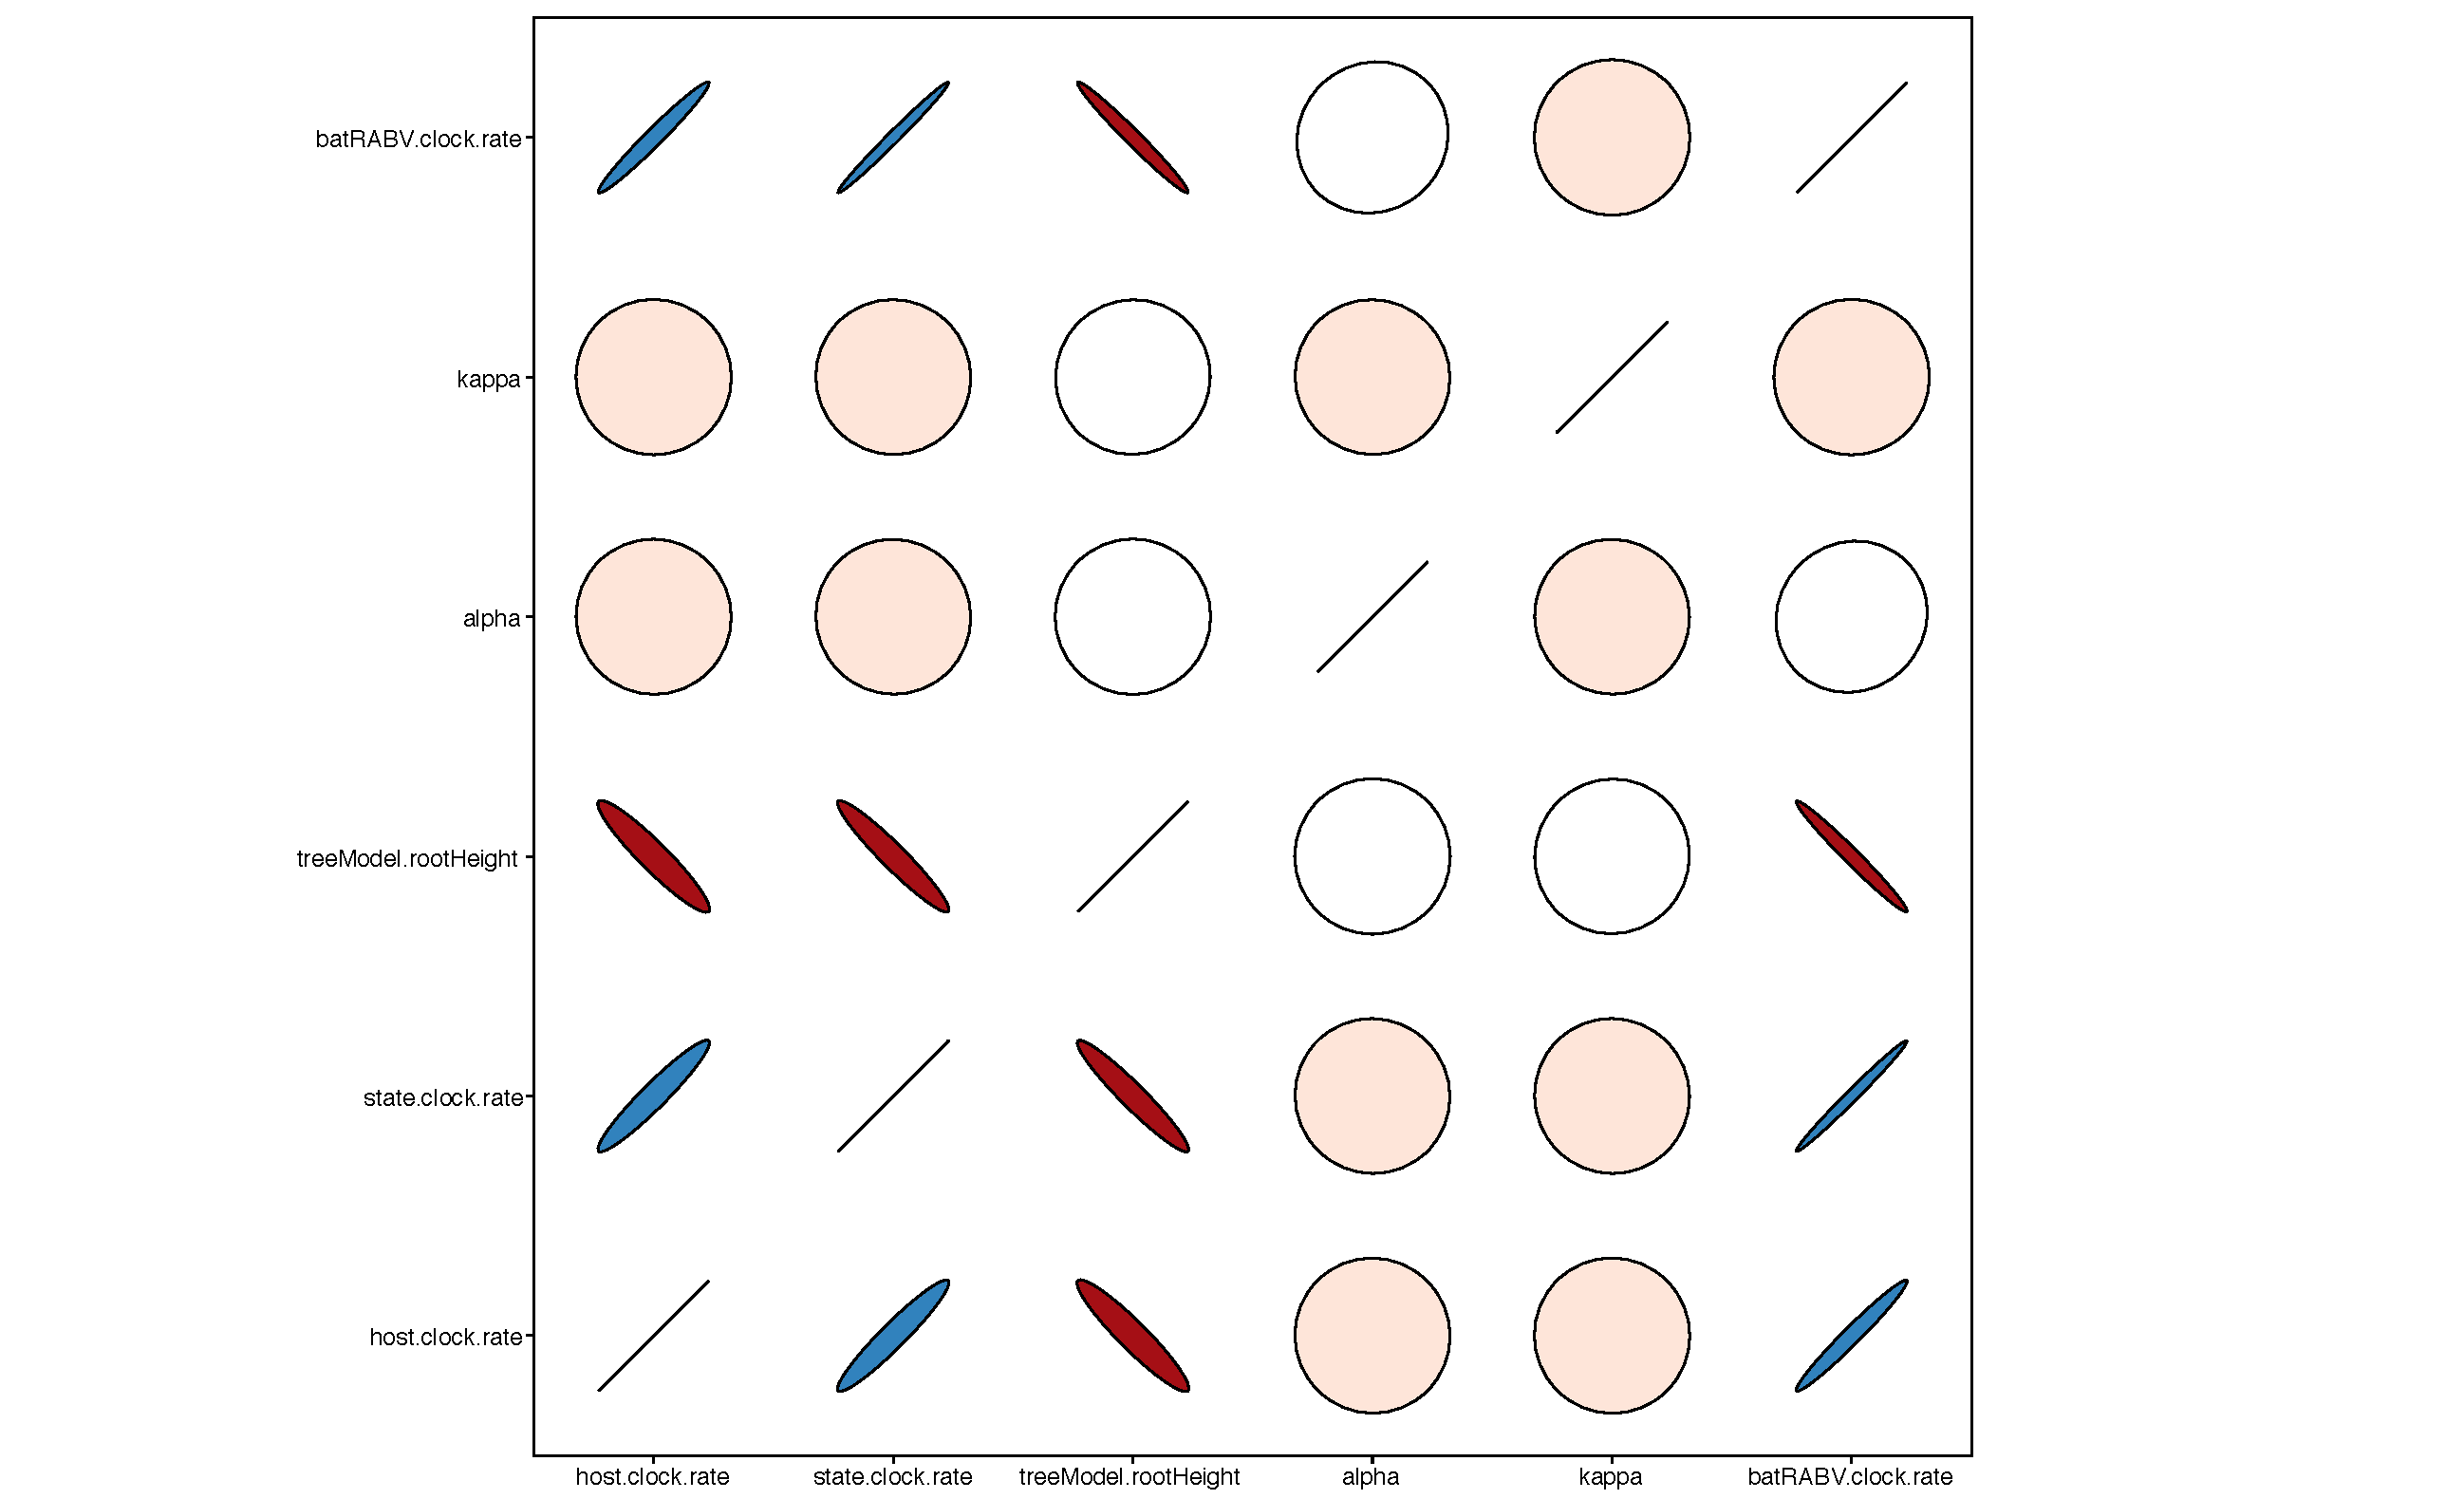
\includegraphics[width = .23\textwidth, height = 3cm]{./figures/rabv-joint-real.pdf}}
\vspace{-0.25cm}
%\subfigure[Box-and-whisker plot]{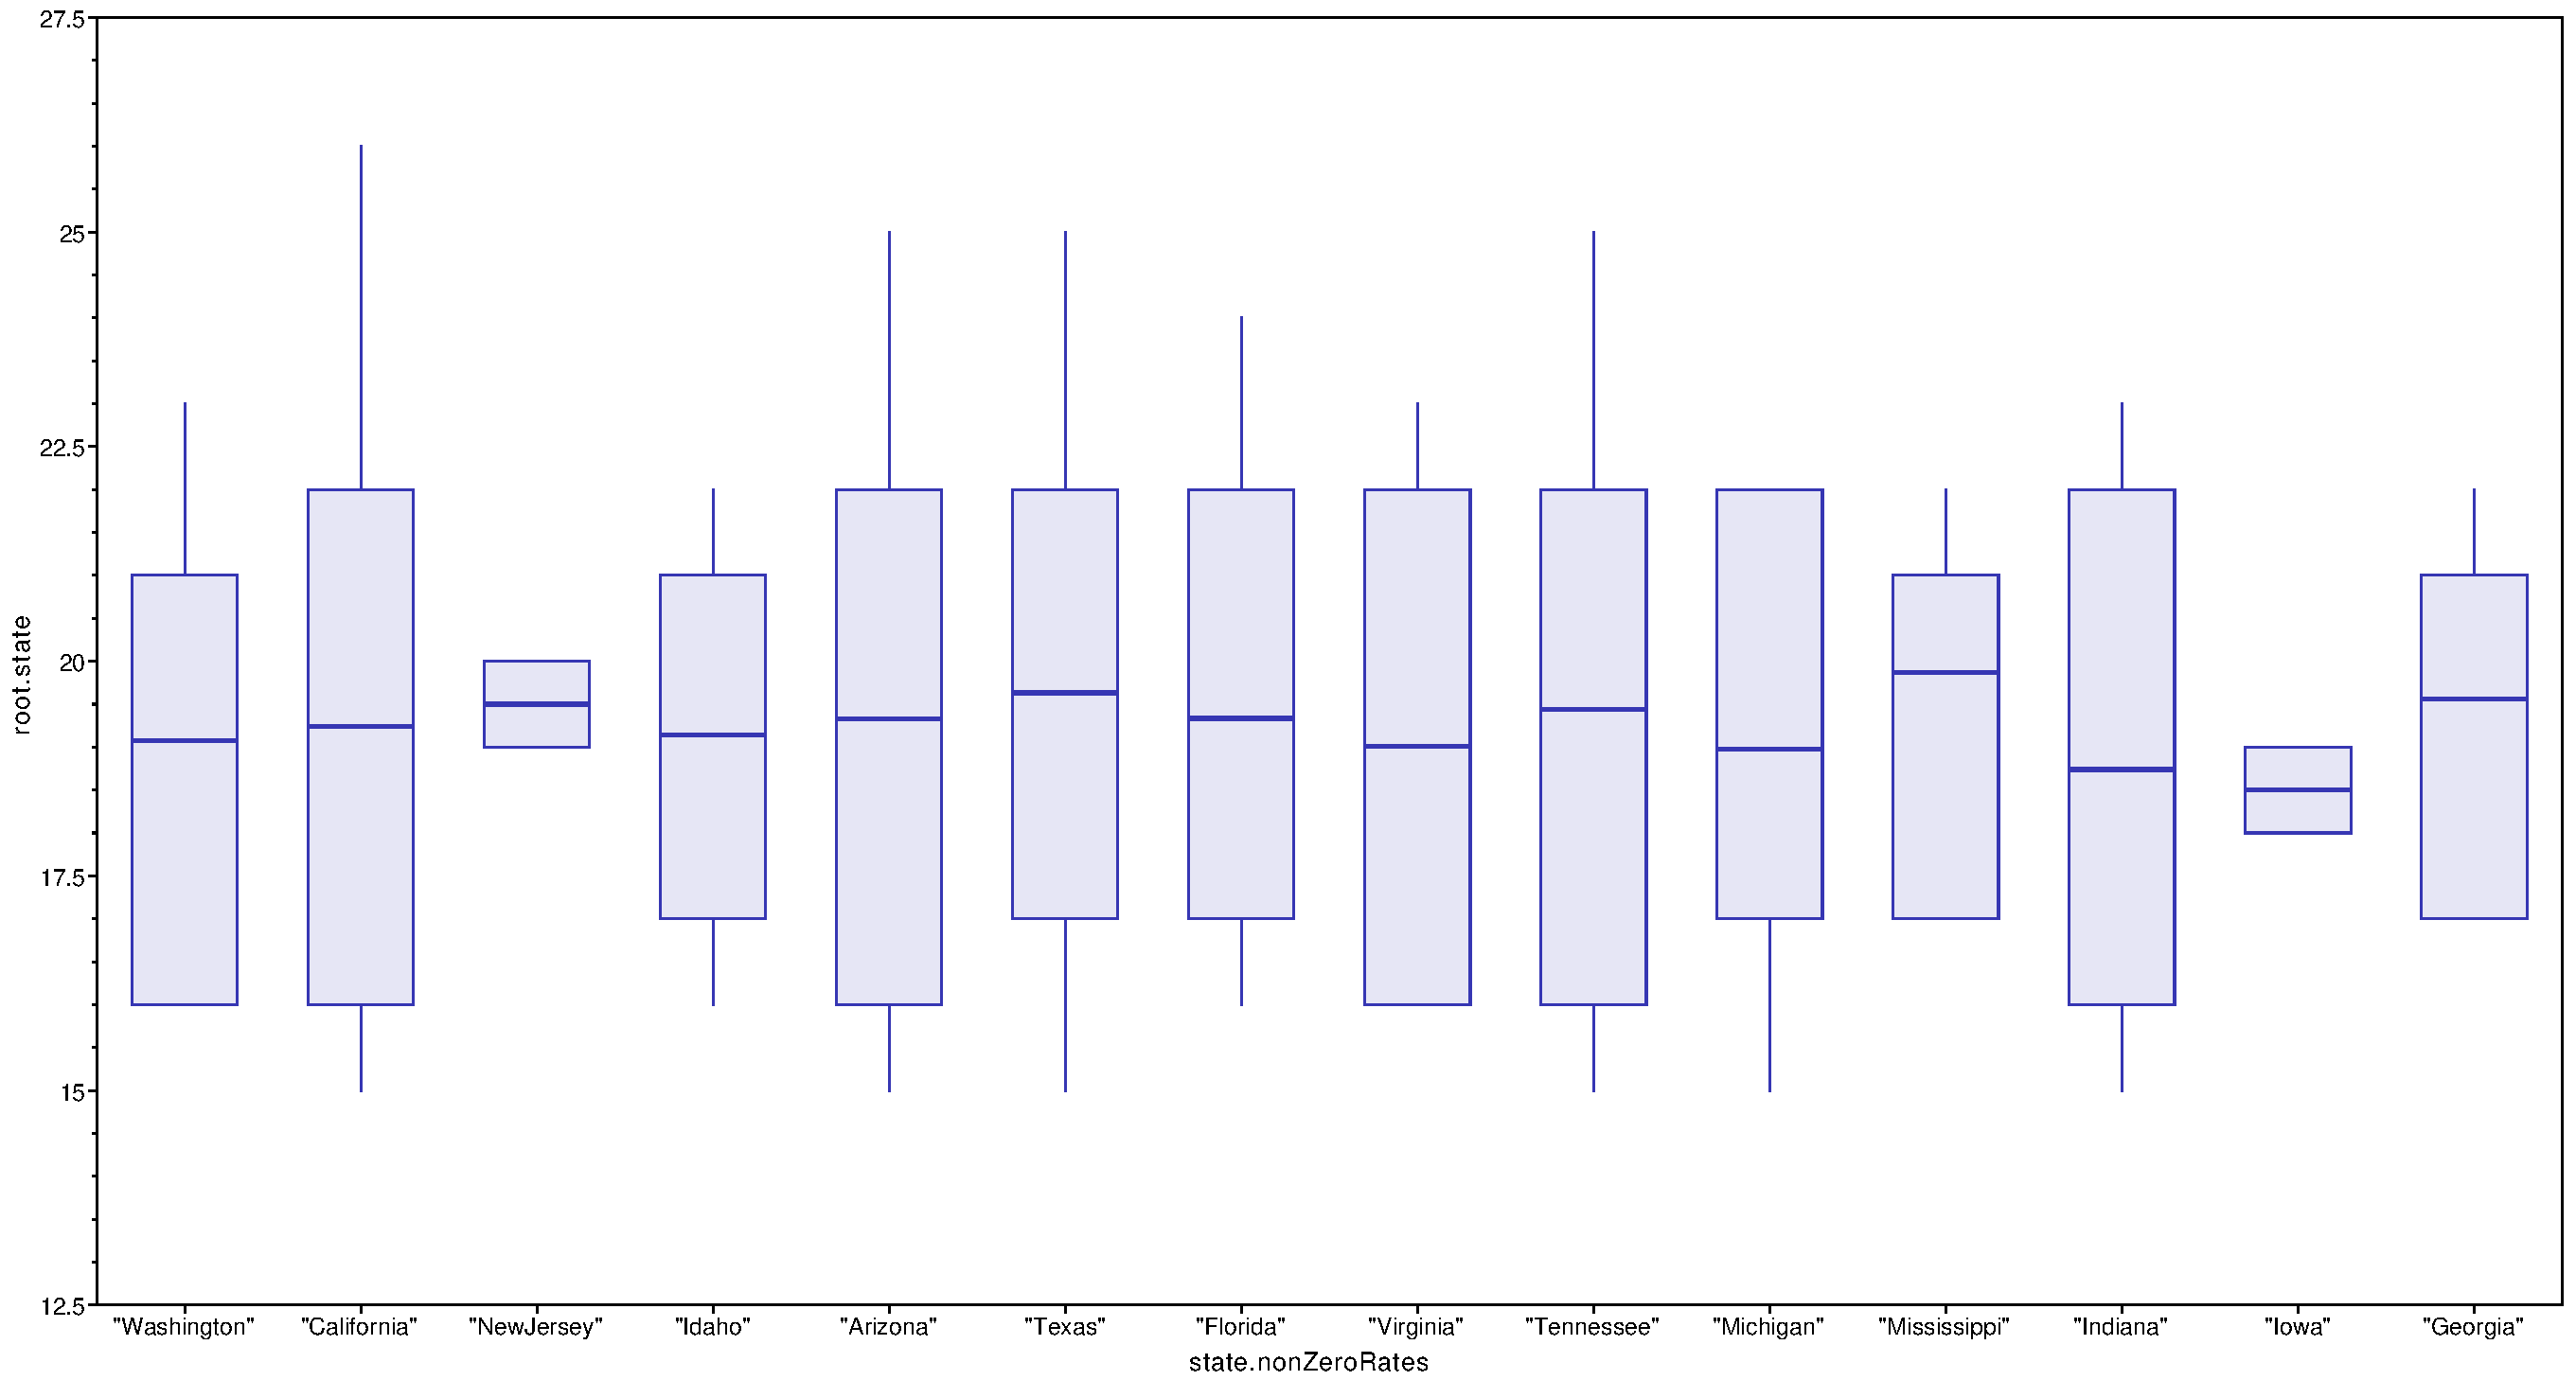
\includegraphics[width = .465\textwidth, height = 3cm]{./figures/rabv-catreal.pdf}}
\caption{Multi-parameter visualisations of: (a) the joint probability distribution of two integer variables through a bubble chart; (b) the marginal density of multiple integer or categorical variables through frequency plots; (c) two continuous variables through a classic scatter or correlation plot; (d) multiple ($> 2$) continuous variables using large correlation matrices.
%; (e) box-and-whisker plots for the joint marginal distribution of a continuous and an integer or categorical variable.
}
\label{fig:4tabs}
\end{figure}
%

\tracer\ offers a solution of visualising conditional posterior distributions as well.
A typical use case involves Bayesian stochastic search variable selection (BSSVS), a form of model averaging, in which parameters influence the likelihood function only when a specific model is selected by a random indicator function.
Under BSSVS, a posterior estimate of the parameter should only sample values from states where the indicator equals one.
Discrete phylogeographic analyses frequently employ BSSVS due to the potentially large amount of transition rates that need to be estimated \citep{Lemey2009}, but this is also relevant when employing model averaging approaches such as for relaxed molecular clocks for example \citep{Li2012}.
%
Finally, \tracer\ provides demographic reconstruction resulting in a graphical plot, often applied to reconstruct epidemic dynamics.
%Depending on the actual demographic model used in the analysis, an additional file containing samples from the posterior tree distribution will be required.
%The currently
Available models are constant size, exponential and logistic growth \citep{drummond2002estimating},
and the non-parametric Bayesian skyline \citep{drummond2005bayesian,heledDrummond2008}, skyride \citep{minin2008smooth} and skygrid \citep{gill2012improving}.
%Not sure if the statement below is correct ...
%All of these demographic models are available in BEAST \citep{drummond2012bayesian} and BEAST2 \citep{bouckaert2014beast2}.
%Besides these, ``Lineages Through Time'' (?) is also available to plot the quantiles of the number of lineages against time, which describes the change of diversification of all organisms over time. %citation?

\vspace{-0.5cm}

\section*{Example}

\subsection*{Cross-species dynamics of rabies in North American bats}

We use \tracer\ to infer the spatial dispersal and cross-species dynamics of rabies virus (RABV) in North American bats.
The data set comprises 372 \textit{nucleoprotein} gene sequences from 17 bat species, sampled between 1997 and 2006 across 14 states in the United States \citep{Streicker,Faria2013}.
%We estimate the ancestral locations of RABV and their host-jumping history using a Bayesian discrete phylogeographic approach with BSSVS \citep{Lemey2009}, while simultaneously estimating RABV effective population sizes over time through a Bayesian skygrid coalescent model \citep{gill2012improving}.
We estimate RABV ancestral locations and host-jumping history using a Bayesian discrete phylogeographic approach with BSSVS, while simultaneously estimating effective population sizes over time through a Bayesian skygrid coalescent model \citep{gill2012improving}.

Phylogeographic BSSVS inference includes parameters of both integer (number of non-zero transition rates) and categorical (host or location-state) trace types.
%While a single parameter of such types can easily be visualised using a frequency plot,
In \tracer, a bubble chart visualises the joint probability distribution between two integer or categorical traces (see Figure \ref{fig:4tabs}:a).
Circle area is proportional to the joint probability, %the blue coloured circle is in the credible set of given a probability threshold default to 0.95, the red is in the set not in the credible set.
with a coloured tile background if this probability reaches a nominal threshold to enhance visibility.
%The coloured background can also help to show the area of the credible set and non-credible set.
%Multiple integer parameters can also be visualised using
Marginal density plots can also display multiple integer parameters, each with unique colour scales (see Figure \ref{fig:4tabs}:b).
With approximately equal numbers of transition rates, both figures suggest similar host and location trait model complexity.
%Both figures show a clear overlap in the number of non-zero transition rates in the discrete trait models for host and location, as identified using a BSSVS procedure.
\tracer\ also provides
%The visualisation options for integer or categorical parameters are complemented with
 popular visualisations for continuous parameters, including scatter plots for two parameters (see Figure \ref{fig:4tabs}:c),
 and extensions for correlations between $\ge\hspace{-0.32em}2$ continuous parameters (Figure \ref{fig:4tabs}:d; \citet{Murdoch}).
 %, which indicates a strong positive correlation between the clock rates of both discrete trait models.
%We also provide an extension of such a scatter plot for multiple (i.e. more than two) continuous variables (see Figure \ref{fig:4tabs}:d; \citet{Murdoch}), which makes use of coloured ellipses to indicate the strength of correlation between each pair of continuous variables.
Colour gradients indicate strength and direction of the correlation, from red (strong negative) to blue (strong positive).
%with a colour gradient from white to dark blue indicating increasingly strong correlation and a colour gradient from white to dark red indicating increasingly strong anti-correlation.
Ellipse shapes re-enforce the strength of correlation, with no correlation appearing as a circle and perfect (anti-)correlation as a line.
%Finally, in order to display the joint marginal distribution between a continuous variable and an integer or categorical variable, we make use of box-and-whisker plots.
%Using such a plot (Figure \ref{fig:4tabs}:e), we can infer that the range of the non-zero transition rates can depend on the ancestral location state inferred at the root of the underlying phylogeny.

\tracer\ reconstructs the demographic history of RABV by drawing the effective population sizes over time (Figure \ref{fig:rabv}).
%Given the properties of this coalescent prior, which requires to specify a grid of intervals over the timeframe of the epidemic, \tracer\ is able to infer this history without requiring a posterior sample of trees.
%According to \tracer's skygrid plot, it is clear that
RABV has successfully established itself in North American bat species, with its effective population size rising steadily throughout recent centuries.
Following a rapid decline at the end of last century, we observe a recent sharp increase in size.
%, reflecting [INSERT SOMETHING].

\begin{figure}[t]
\centerline{
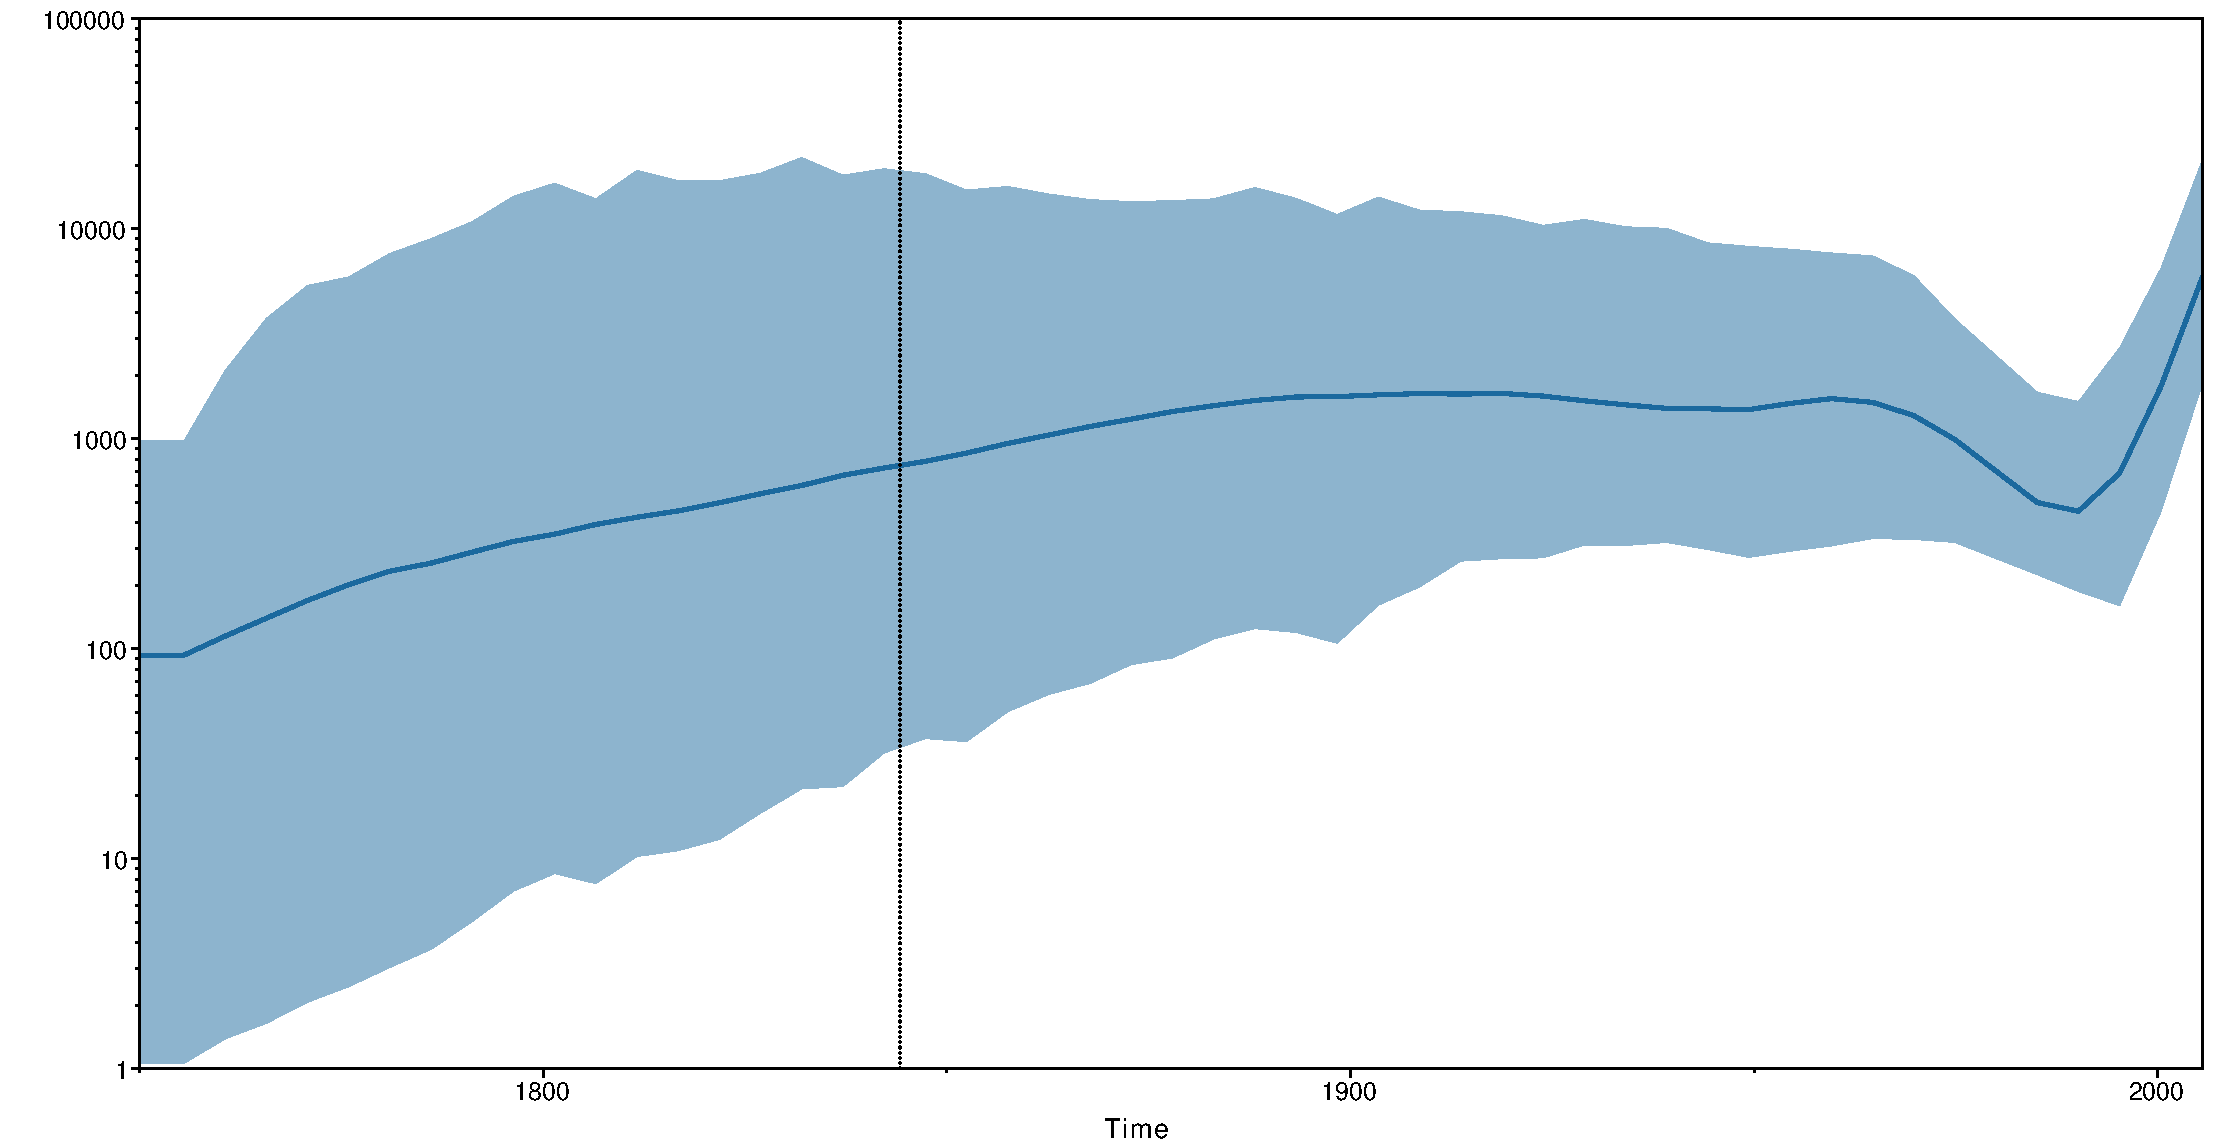
\includegraphics[width=0.46\textwidth]{./figures/rabv-skygrid.pdf}
}
\vspace{-0.25cm}
\caption{Estimating the effective population sizes over time using a Bayesian skygrid demographic reconstruction for rabies virus in North America.}
\label{fig:rabv}
\end{figure}


%Other packages for post-processing of MCMC samples are 

Other packages are available for the post-processing of MCMC samples. % and are largely complementary to \tracer\ .
 `Coda' \citep{plummer2006coda} provides some of the functionality of \tracer\ within the R programming environment, while `AWTY' \citep{nylander2007awty} explores the convergence of the phylogenetic tree parameter itself across multiple MCMC runs.
%% AR - anything else? The MDS tree-space approaches of Hillis etc.?

\vspace{-0.35cm}

\section*{Availability}

\tracer\ is open-source under the GNU lesser general public license and available in both source code (\url{https://github.com/beast-dev/tracer}) and executable (\url{http://beast.community/tracer}) forms.
This latter page also serves up self-contained, step-by-step tutorials covering basic to advanced usage of \tracer\ to summarise posteriors under a variety of phylogenetic models using BEAST.
Popular tutorials employ \tracer\ to generate marginal parameter summaries and to infer population dynamics trajectories over time.
\tracer\ requires Java version 1.6 or greater.



%\section*{Old Text}
%
%%You can also select the "Demographic Analysis" from the Analysis menu - This plots the distribution of demographic population sizes over time for a number of models (constant size, exponential growth \& logistic growth) that are available in BEAST. This involves you selecting the traces for each parameter of the model. You should only select the model that was actually run under BEAST (e.g., if you ran an exponential growth model, you shouldn't plot the constant population size model).
%
%%The "Analysis" menu also contains options for performing Bayesian Skyline reconstructions and for calculating Bayes Factors between runs.
%
%Feature list:
%\begin{itemize}
%\item KDEs
%\item cheap marginal likelihood estimators
%\item demographic trajectory reconstruction
%\end{itemize}
%
%%Model selection HME and AICM have been removed
%New features:
%\begin{itemize}
%\item Three trace types: real, integer, string
%\item Kernel density estimates
%\item Conditional posterior distribution
%%\item HME
%%\item AICM
%\end{itemize}
%
%%\begin{figure}[H]
%%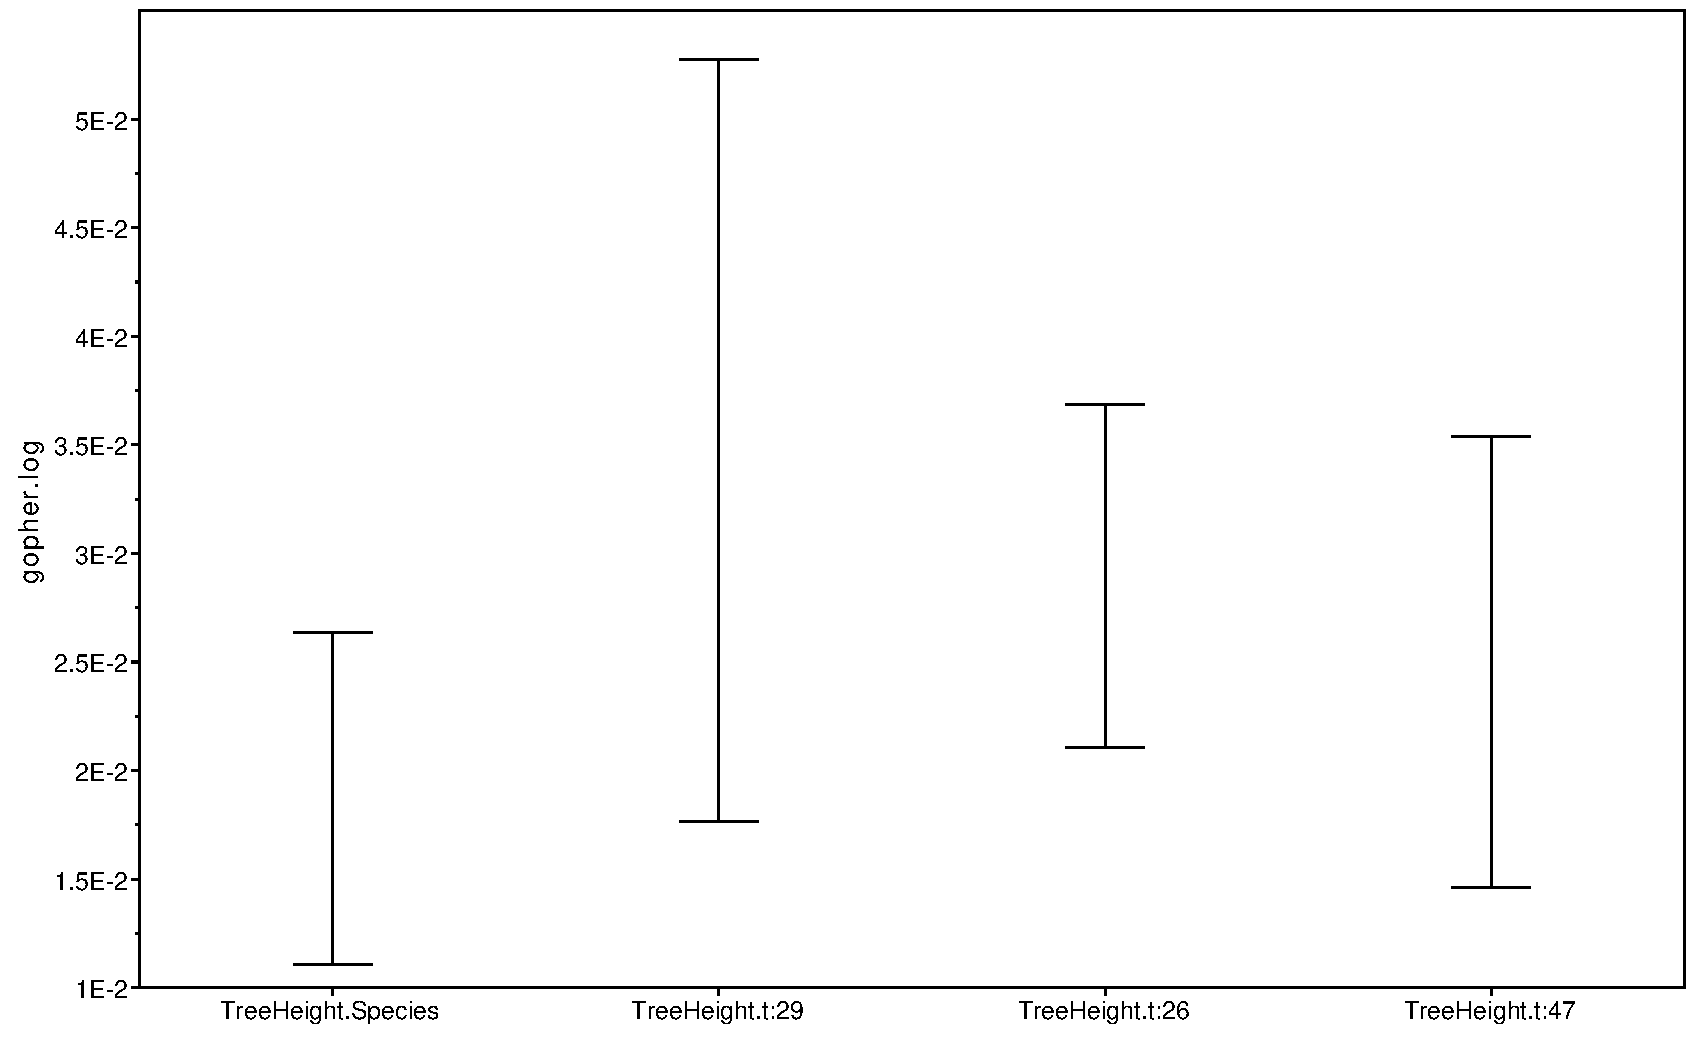
\includegraphics[width=.5\textwidth]{./figures/comp-95HPD.pdf}
%%\caption{The comparison of  95\% HPD intervals from multi-trace}
%%\label{fig:comp95HPD}
%%\end{figure}
%
%%\begin{figure}[H]
%%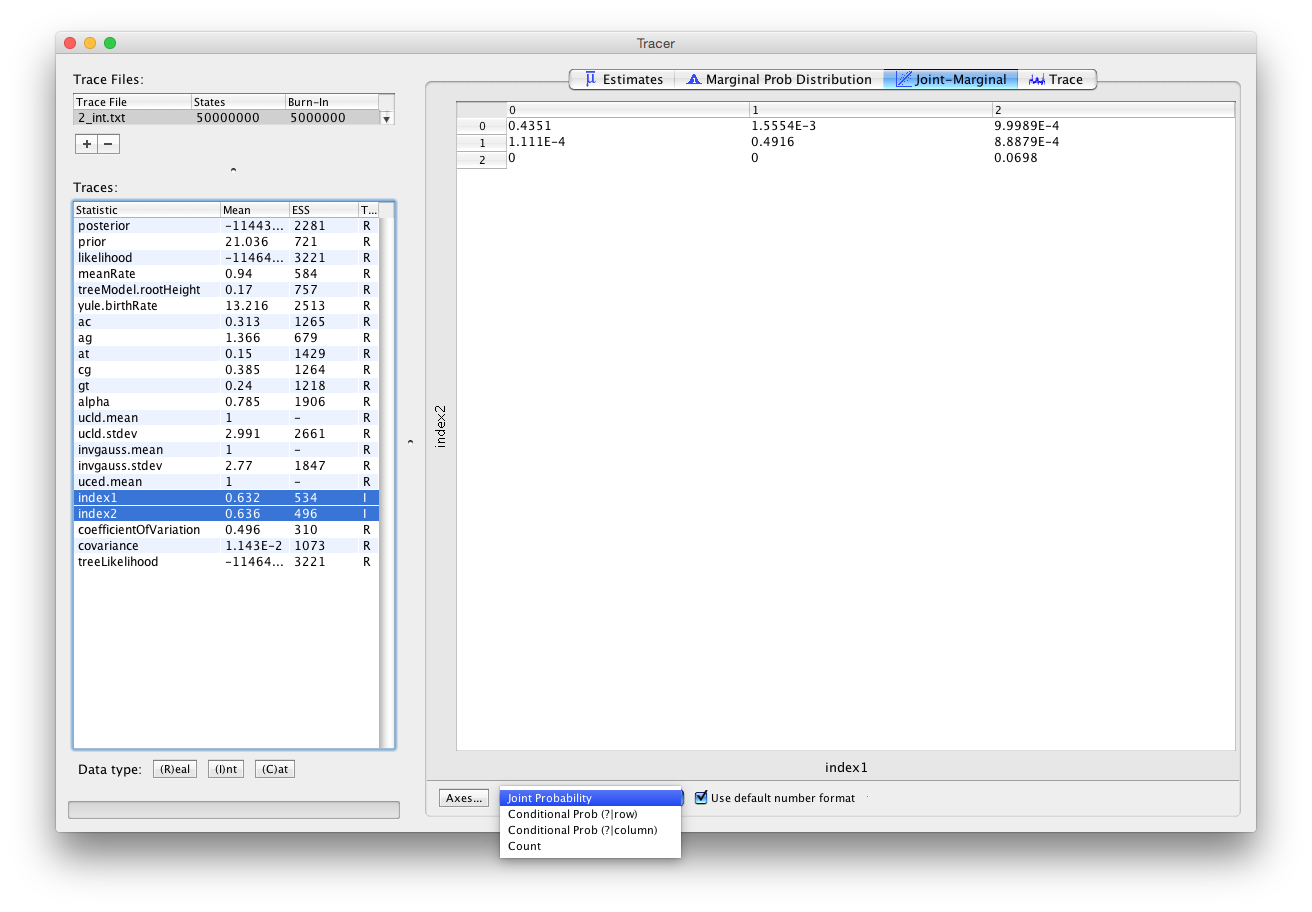
\includegraphics[width=.5\textwidth]{./figures/jointPrInt.png}
%%\caption{The Joint probability table of two integer traces}
%%\label{fig:int:jointpr}
%%\end{figure}
%
%%\begin{figure}[ht]
%%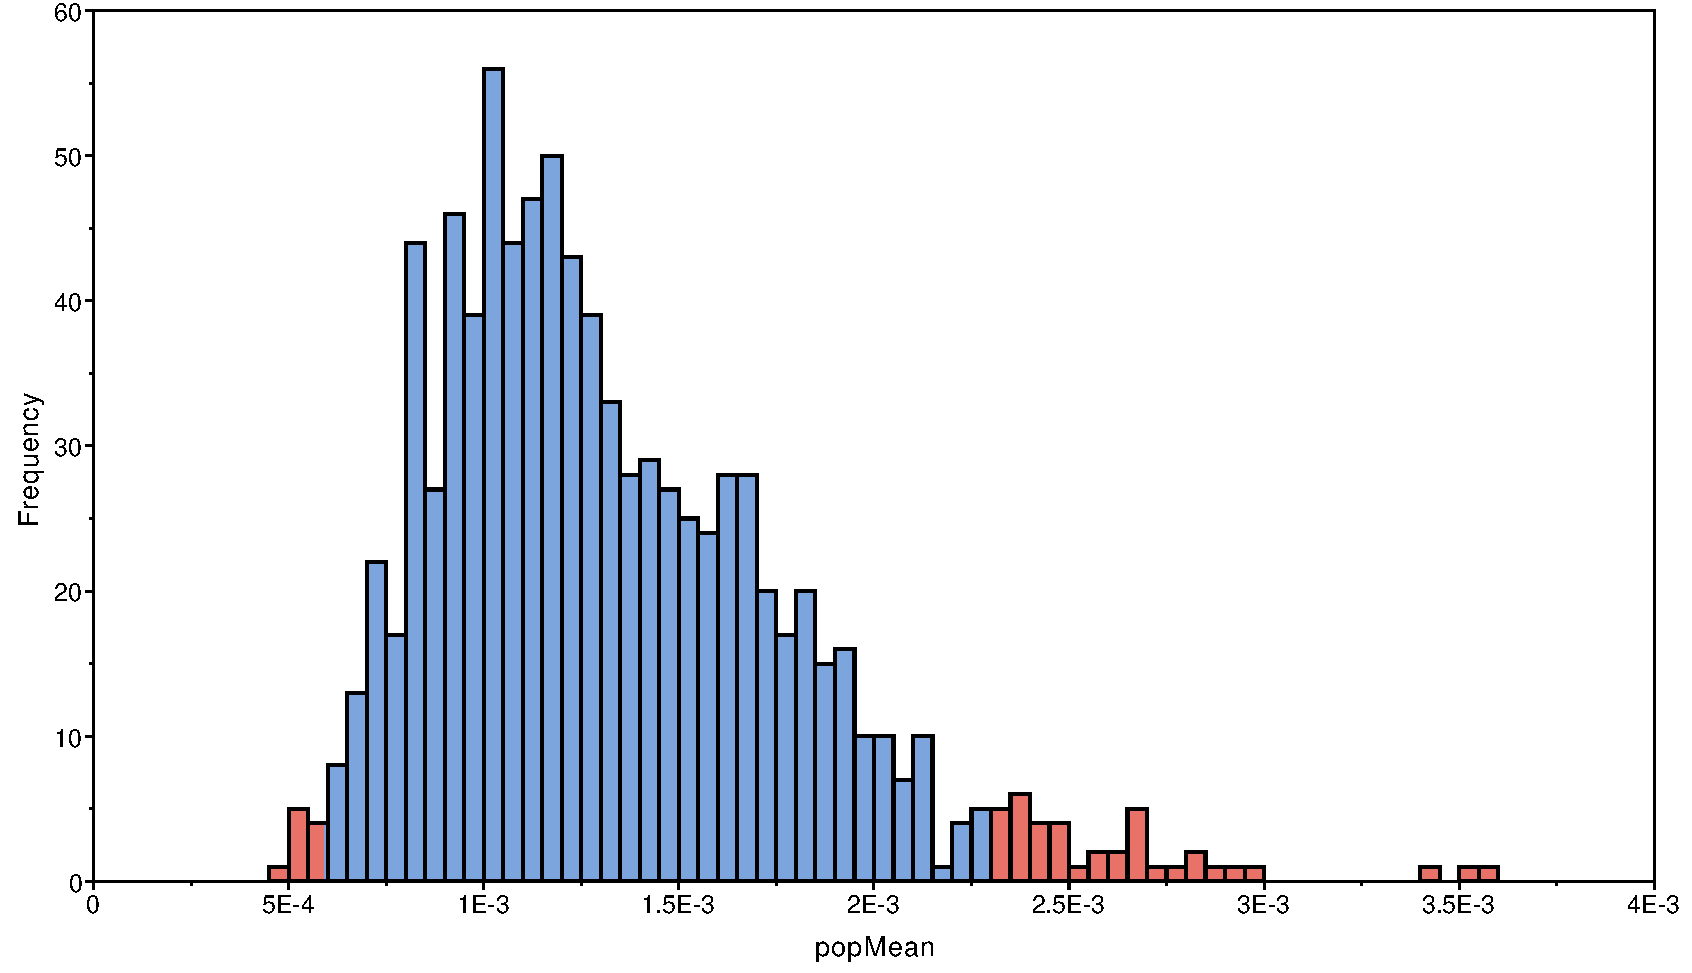
\includegraphics[width=.5\textwidth]{./figures/frequency.pdf}
%%\caption{A frequency distribution for a continuous trace}
%%\label{fig:freq}
%%\end{figure}
%%\begin{figure}[ht]
%%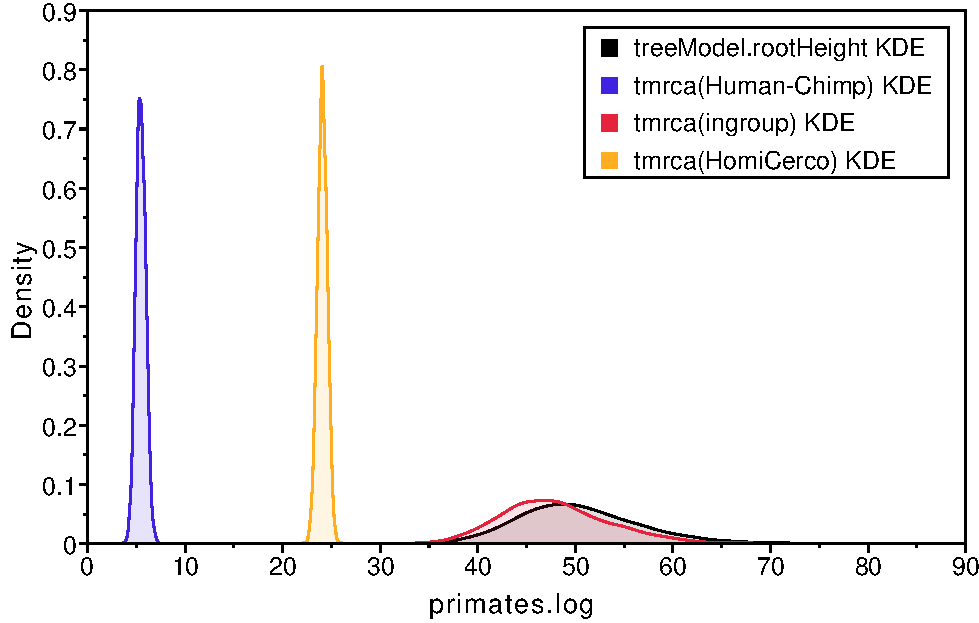
\includegraphics[width=.5\textwidth]{./figures/multiKDE.pdf}
%%\caption{KDE of multiple traces}
%%\label{fig:multiKDE}
%%\end{figure}
%%\begin{figure}[ht]
%%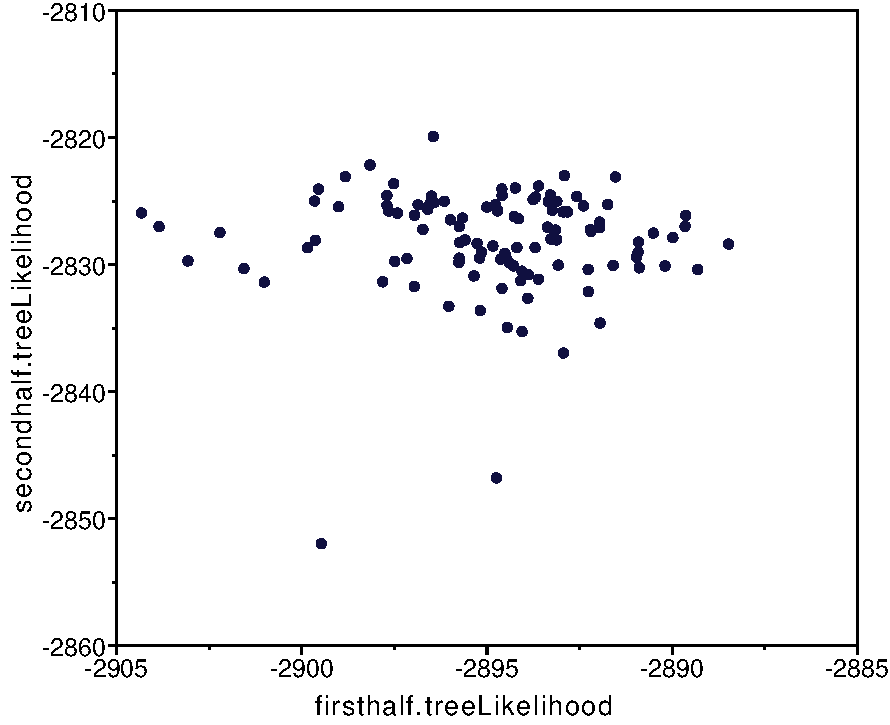
\includegraphics[width=.5\textwidth]{./figures/joint-marginal.pdf}
%%\caption{The joint-marginal distribution of two selected tes}
%%\label{fig:trace}
%%\end{figure}
%%\begin{figure}[ht]
%%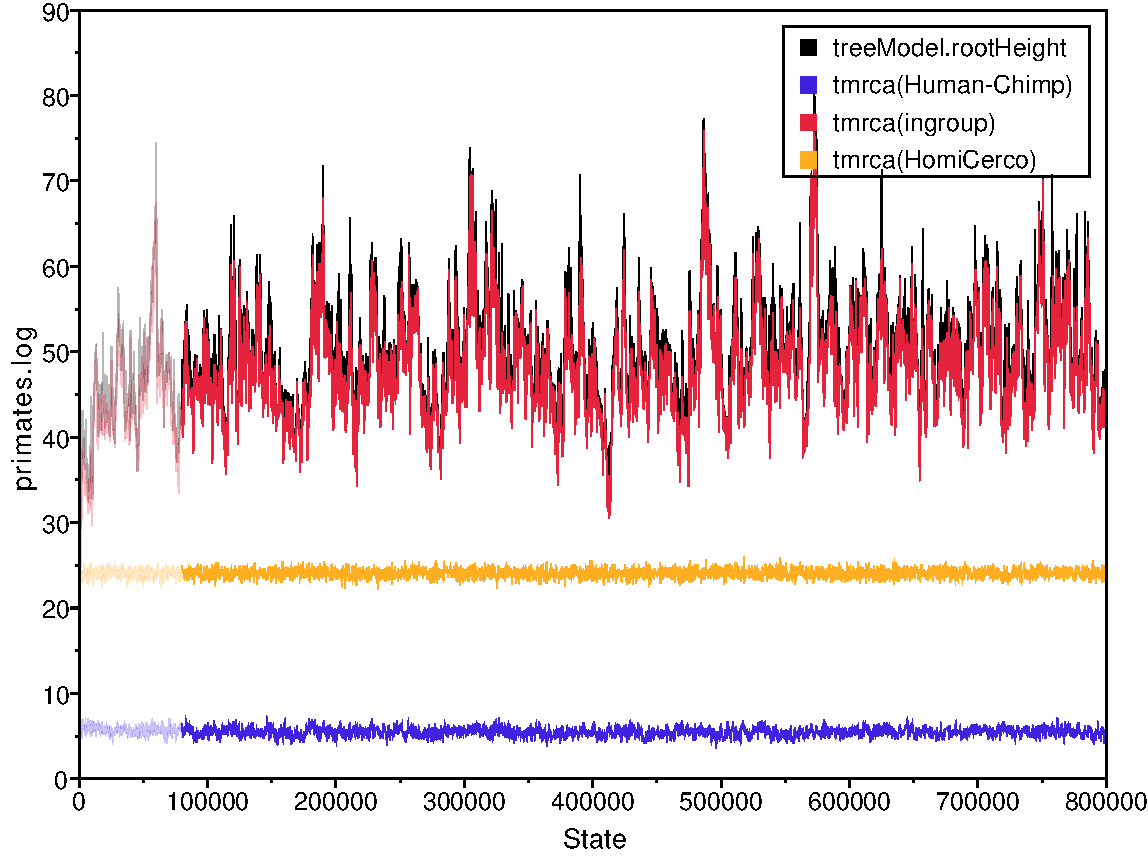
\includegraphics[width=.5\textwidth]{./figures/trace.pdf}
%%\caption{The selected traces against state}
%%\label{fig:trace}
%%\end{figure}
%
%
%\subsubsection*{Diagnostics:} Blah blah
%
%\subsubsection*{Demographic reconstruction:}
%
%%\subsubsection*{Model selection:}
%
%\subsubsection*{Conditional posterior distribution:}

%Fairly general solution to looking at conditional posterior distributions;

%Specifically, support for BSSVS forms of model averaging, in which some parameters are only in the likelihood when their submodel is "indicated" by some indicator function that is usually a discrete, integer or boolean variable. In that case the posterior of the parameter should not include the states when it was sampled only in the prior because the submodel it belonged to was "turned off". This is relevant for EBSP, Random Local Clocks model, microsatellite model averaging and relaxed clock model averaging methods all from my group in last couple of years. Also relevant for BSSVS in phylogeography as well depending on how the state is logged.
%\section*{Taken from the Tracer website}

%Tracer is a program for analysing the trace files generated by Bayesian MCMC runs (that is, the continuous parameter values sampled from the chain). It can be used to analyse runs of BEAST \citep{drummond2012bayesian,drummond2012bayesian}, BEAST2 \citep{bouckaert2014beast2}, MrBayes \citep{ronquist2012mrbayes}, RevBayes \citep{hohna2016revbayes}, LAMARC \citep{kuhner2006lamarc}, Migrate \citep{beerli2006comparison} and possibly other MCMC programs.

%Although Tracer can be used with programs other than BEAST, users may find it useful to join the BEAST users mailing list. This is used to announce new versions and advise users about bugs and problems.

%You can join the mailing list here:
%http://groups.google.com/group/beast-users

%The website for BEAST (and Tracer) is here:
%http://beast.bio.ed.ac.uk/

%At present there is no detailed manual for this application, you will simply have to play around and see what happens. Basically you can select the trace file in the top left of the window, the individual parameter in the bottom left and the analysis appears on the right.

%There are 4 analysis tabs to choose from:

%Estimates - this shows the mean, stdev, confidence intervals and other statistics about the selected parameter. A frequency distribution will also be plotted.
%Density - this shows the Bayesian posterior density plot for the selected parameter.
%Joint-Marginal - this only appears if exactly 2 parameters are chosen (hold down shift to select multiple parameters). It then plots one against the other to look at their joint-marginal distribution.
%Trace - this shows the trace of the parameter against state or generation number. Use this to check mixing, choose a suitable burn-in and look for trends that might suggest problems with convergence.
%Multiple parameters can be selected by holding down the shift key. This will overlay the plots for the different parameters allowing comparisons to be made. You can also select multiple trace files as well to compare different runs. If multiple trace files have the same trace names then a "Combined" trace will automatically appear. This can be selected as well as the individual trace files.

%You can also select the "Demographic Analysis" from the Analysis menu - This plots the distribution of demographic population sizes over time for a number of models (constant size, exponential growth \& logistic growth) that are available in BEAST. This involves you selecting the traces for each parameter of the model. You should only select the model that was actually run under BEAST (e.g., if you ran an exponential growth model, you shouldn't plot the constant population size model).

%The "Analysis" menu also contains options for performing Bayesian Skyline reconstructions and for calculating Bayes Factors between runs.

%The "Print" function in the "File" menu will print the current graph or table and the "Export Data" function can be used to export the data from the plots for use in another graphic package.

%To export the currently displayed graphic use the "Export PDF" function in the "File" menu.

\vspace{-0.35cm}

\section*{Acknowledgements}

This work was supported in part by the Wellcome Trust through project 206298/Z/17/Z (Artic Network), the European Union Seventh Framework Programme under grant agreement no. 725422-RESERVOIRDOCS, the National Science Foundation through grant DMS 1264153, the National Institutes of Health under grants R01 AI107034 and U19 AI135995. AJD acknowledges support from Marsden grant contract UOA1611.
GB acknowledges support from the Interne Fondsen KU Leuven / Internal Funds KU Leuven.


\vspace{-0.35cm}

%\section*{References}
% The bibtex filename
\bibliographystyle{natbib}
\bibliography{tracer17}

\end{document}

